\chapter{Modelos de aprendizaje profundo}
\label{ANNs}

%\section{Teoría sobre redes neuronales}
%\section{Estructura de las redes}
% He considerado tres modelos diferentes de redes neuronales: 
% \begin{itemize}
%     \item Modelo denso: Consta de dos capas densas (Fig. \ref{Red_densa})
%     \item Modelo LSTM1: Consta de una capa compuesta por una red recurrente con memoria (LSTM) y una capa densa 
%     \item Modelo LSTM2: Dos capas LSTM y una capa densa
% \end{itemize}
\section{Introducción teórica}

Las redes neuronales son modelos computacionales cuyo funcionamiento se inspira en el funcionamiento de las 
neurona cerebrales reales, su función principal es recibir, procesar y transmitir información a través de señales
químicas y eléctricas. En líneas generales, las neuronas se especializan en la recepción de estímulos y generación
de impulsos entre ellas mediante conexiones llamadas sinapsis. Cuando una neurona recibe un impulso 
eléctrico que la activa, esta dispara un impulso que a su vez estimula a otras neuronas a las que está conectada. 
Algunas de estas neuronas a su vez se activan y se disparan activando a otras y así sucesivamente 
propagando los estímulos por toda la red. Entre más se practique una tarea, las conexiones que se generan entre las 
neuronas se hacen más robustas, esto es el proceso de aprendizaje. 

\begin{figure}[h!]
    \begin{center}
      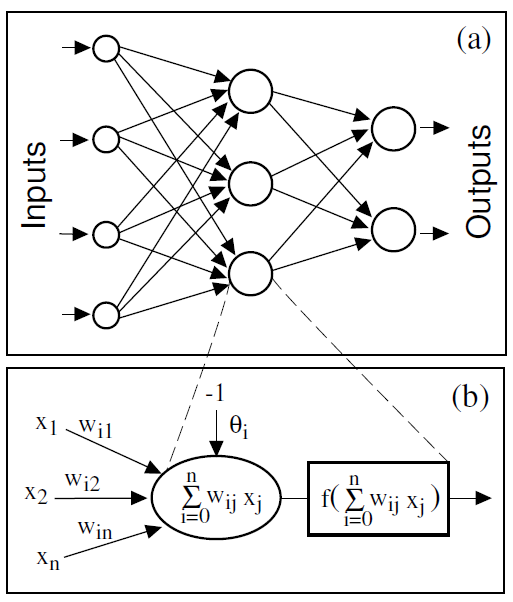
\includegraphics[height=2.5in]{Figures/esquema_red.PNG}
      \caption{ Representación gráfica de una neurona artificial (figura tomada de \cite{gutierrez}). }
      \label{perceptron}
    \end{center}
  \end{figure}

Una neurona artificial (Fig. \ref{perceptron}-b) funciona de una manera muy similar a las neuronas biológicas, 
ésta recibe datos de entrada que son combinados por la neurona asignando pesos a cada uno de ellos, a los 
cuales se aplica una función de activación que activa a la neurona si esta supera un umbral 
dado. La función de activación además de cumplir la función de activar a las neuronas, capta las 
características no lineales de los datos. 

Una red neuronal (ANNs, de sus siglas en inglés) consiste de un conjunto de neuronas conectadas entre sí 
(Fig. \ref{perceptron}-a), que al igual que en el caso de las neuronas reales son capaces de ser entrenadas para aprender 
a realizar una tarea dada generando diferentes conexiones entre ellas. 

\begin{figure}[h!]
    \begin{center}
      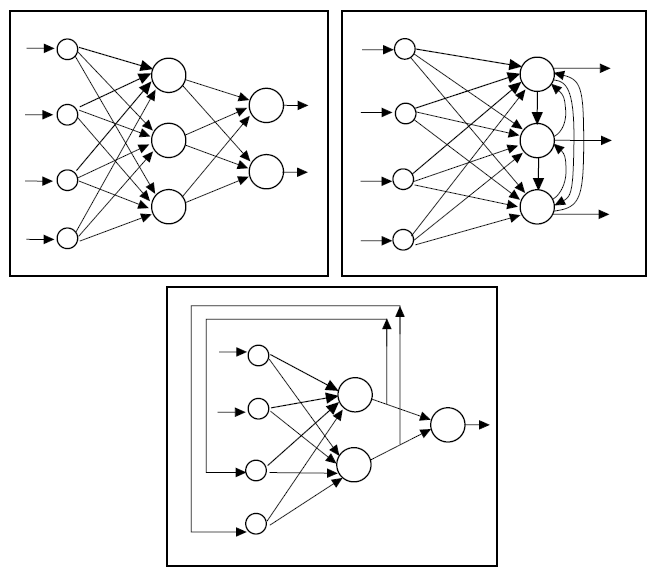
\includegraphics[height=2.5in]{Figures/topologias.PNG}
      \caption{ Tres topologías distintas de red neuronal: (a) multicapa, (b) competitivas, (c) recurrentes. }
      \label{topologias}
    \end{center}
  \end{figure}

La estructura de la red puede tener distintas topologías, en la figura \ref{topologias} se muestran tres modelos de red neuronales 
distintos: \textit{re multicapa} que solo tiene conexiones entre neuronas de capas consecutivas, 
\textit{red competitiva} que también posee conexiones entre de la última capa y \textit{redes recurrentes} (RNN) que posee conexiones entre 
capas no consecutivas. En este trabajo se han utilizado tanto redes multicapa como redes recurrentes, que son apropiadas para problemas de 
aprendizaje supervisado en donde cada patron de entrenamiento (entrada de la red) $X_p=(x_{1p},...x_{mp})$ tiene asociado un 
correspondiente patrón de salida $Y_p=(y_{1p},...y_{np})$. 
El entrenamiento  se basa en que la red sea capaz de reproducir los patrones de salida con el menor error posible.

El proceso de aprendizaje de la red consiste en la aplicación de métodos de optimización matemáticos para obtener los pesos $w_{ij}$ 
que minimizan una cierta función de coste o \textit{loss}. Los algoritmos más populares se basan en minimizar el error cuadrático 
medio (RMSE):

\begin{equation}
    E(w) = \sum_{j,p}(y_{jp}-\hat{y}_{jp})^2
\end{equation}

Uno de los algoritmos más simples es el de descenso de gradiente que en cada etapa intenta modificar los pesos de forma incremental de manera 
de minimizar la función de loss. El incremento de los pesos se obtiene en base al vector opuesto al gradiente del loss,
 que indica la dirección en la que la función decrece más rápidamente:

 \begin{equation}
    \Delta w_ij = -\alpha \frac{\partial E(w)}{\partial w_ij}
\end{equation}

donde $\alpha$ es la tasa de aprendizaje. 


\begin{figure}[h!]
    \begin{center}
      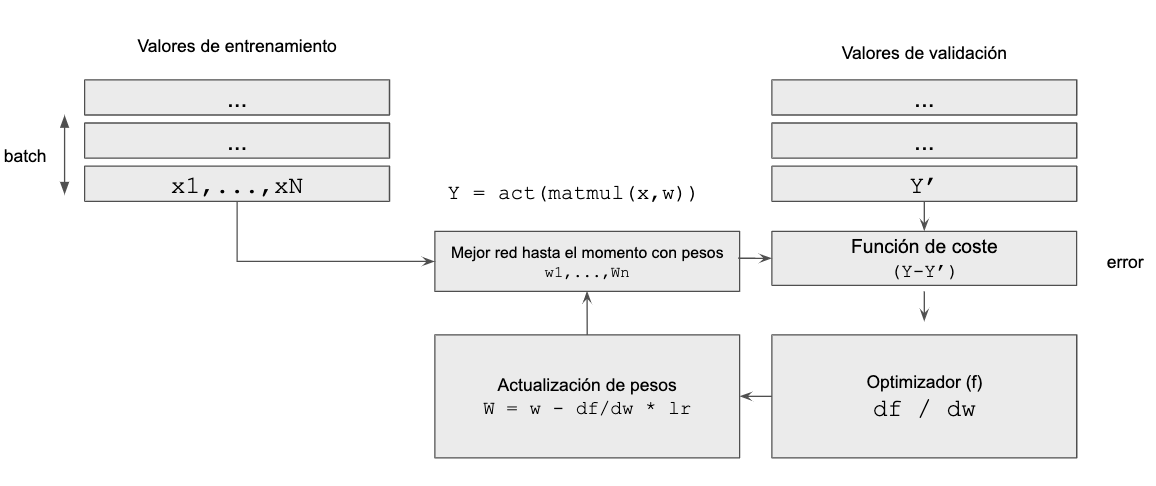
\includegraphics[height=2.in]{Figures/back_prop.png}
      \caption{ Back propagation }
      \label{backprop}
    \end{center}
  \end{figure}


El algoritmo de retro-propagación consta de dos pasos, en primer lugar la entrada $X_p$ se propaga hacia adelante, obteniendo el valor
de todas las unidades ocultas y las salidas $\hat{y}_p$ y por lo tanto el error asociado a éstas. Los valores obtenidos se utilizan para actualizar
los pesos de la capa de salida, y éstos se propagan hacia atrás para actualizar los pesos de las capas ocultas. Esto
 se repite para cada patrón de entrenamiento. En el esquema \ref{backprop} se resume todo el proceso.


% Las redes neuronales aprenden a partir de muestras o ejemplos, hacen una operación de propagación hacia adelante,
% calculan la diferencia entre sus respuestas y las respuestas correctas, y corrigen sus parámetos internos (pesos, bias) 
% según esos errores, a través de retropropagación por descenso de gradiente, o algún otro algoritmo de minimización.

% El problema es que la retropropagación es un cálculo "costoso", porque los gradientes de un nodo de cualquier capa intermedia, reciben contribuciones de muchos otros nodos de las capas anteriores. Por eso, corregir cientos o miles de parámetros con cada nuevo ejemplo, hace muy lenta la ejecución.
% Una alternativa es agrupar las muestras en "paquetes" o batches. El error se calcula sobre cada batch como la suma o promedio de errores de sus muestras, y los parámetros se corrigen una sola vez según el error del batch.
% Cuando el tamaño del batch (batch size) es igual a 1, no hay paquetes. Esto se conoce como descenso de gradiente estocástico.
% Cuando el tamaño del batch es mayor que 1 y menor que el total de muestras, se llama Descenso de Gradiente por Mini-batch.
% Cuando todas las muestras forman un sólo batch, se llama Descenso de gradiente por Batch.
\section{Redes recurrentes con memoria a largo plazo}


\begin{figure}[h!]
  \begin{center}
    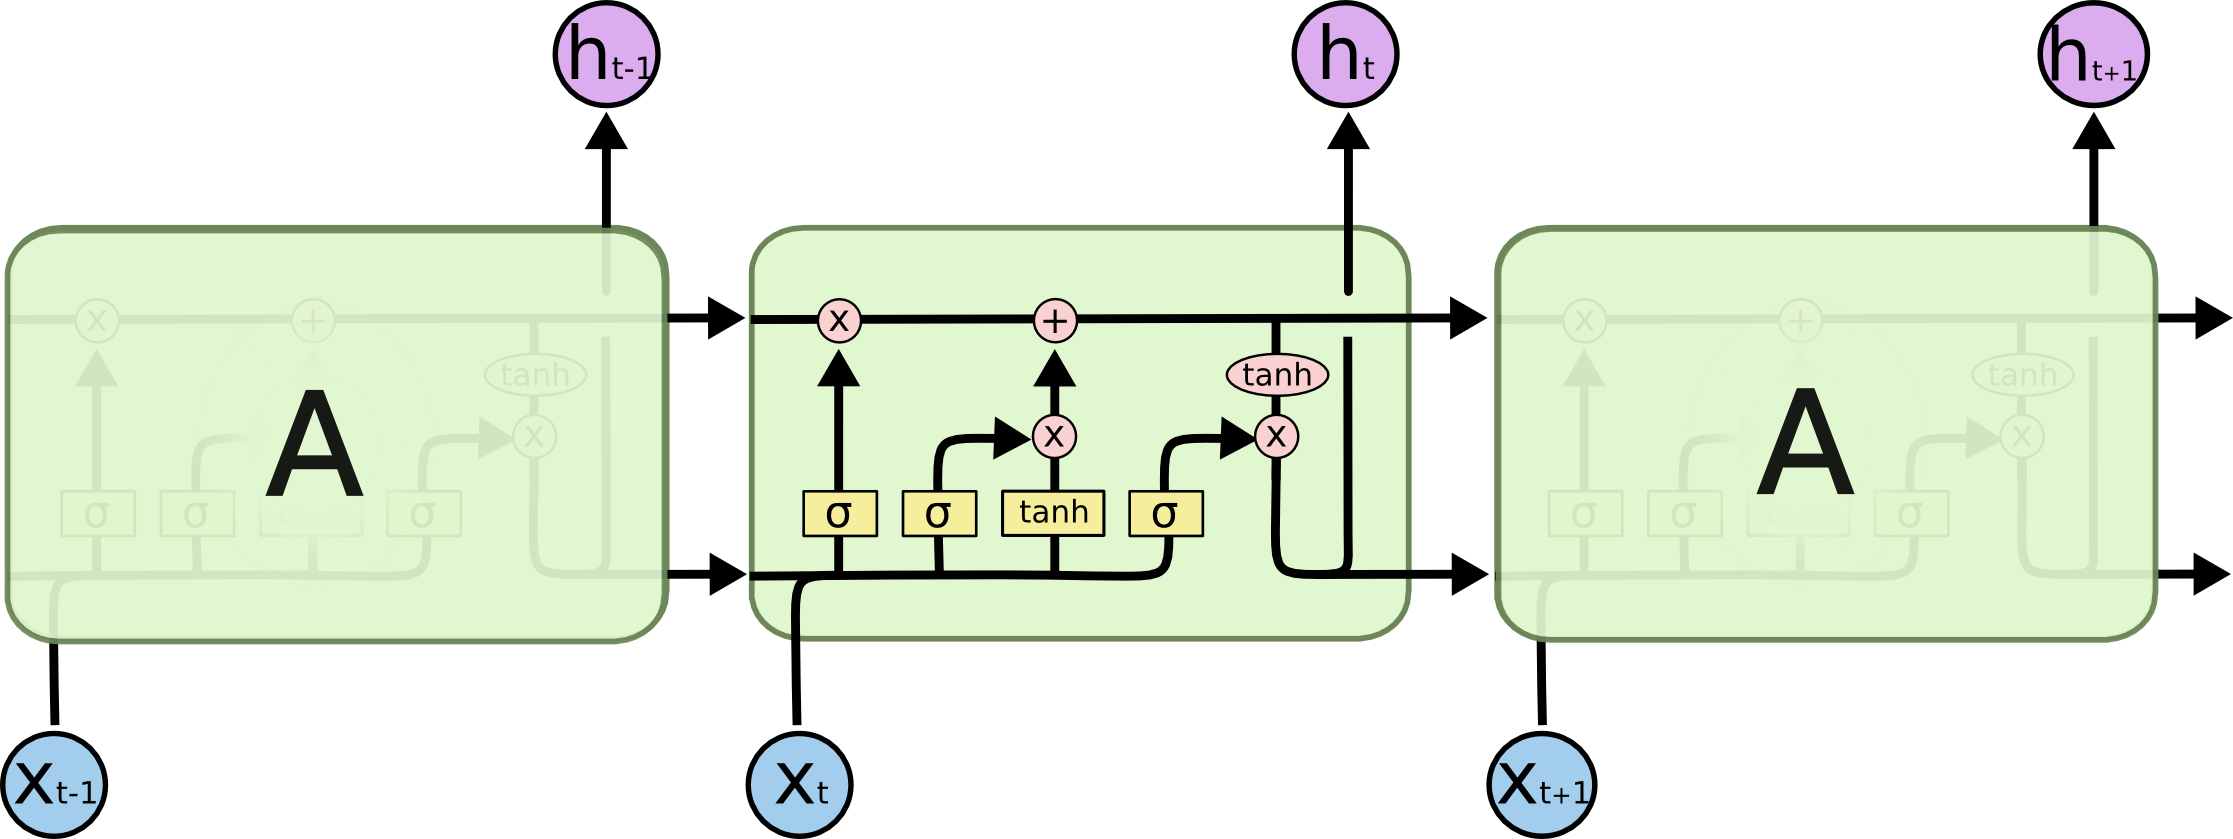
\includegraphics[height=1.8in]{Figures/LSTM3-chain.png}
    \caption{ Red neuronal recurrente con memoria a largo y corto plazo (LSTM). Figura tomada de \cite{olah}. }
    \label{LSTM}
  \end{center}
\end{figure}

Las ANNs recurrentes con memoria a largo plazo (LSTM) son redes que poseen conexiones entre capas 
no consecutivas (Fig. \ref{topologias}-c) que además incluyen una conexión extra entre las neuronas dedicadas
 a almacenar información para largo períodos de tiempo. 
 Esta "memoria a largo plazo" soluciona el problema del desvanecimiento del gradiente que presentan las redes recurrentes 
 tradicionales\cite{Kratzert}, \cite{olah}.

En la figura \ref{LSTM} se puede observar la estructura de una celda de una red LSTM, donde $x_t$ es un input 
dado a un tiempo $t$, $h_t$ el correspondiente output, las celdas amarillas son 
capas de neuronas densas y los círculos rosas son puntos en donde se realiza una cierta operación. La clave en estas
redes es la línea horizontal superior que recorre la cadena casi sin sufrir modificaciones y permite que la información
fluya a través de la red. Mediante las cuatro entradas (celdas amarillas en el esquema),
estas redes poseen la habilidad de eliminar o agregar información al estado de la celda y decidir qué parte de la información
proveniente de capas anteriores es relevante y que parte debe ser olvidada \cite{olah}. 

\begin{figure}[h!]
  \begin{center}
    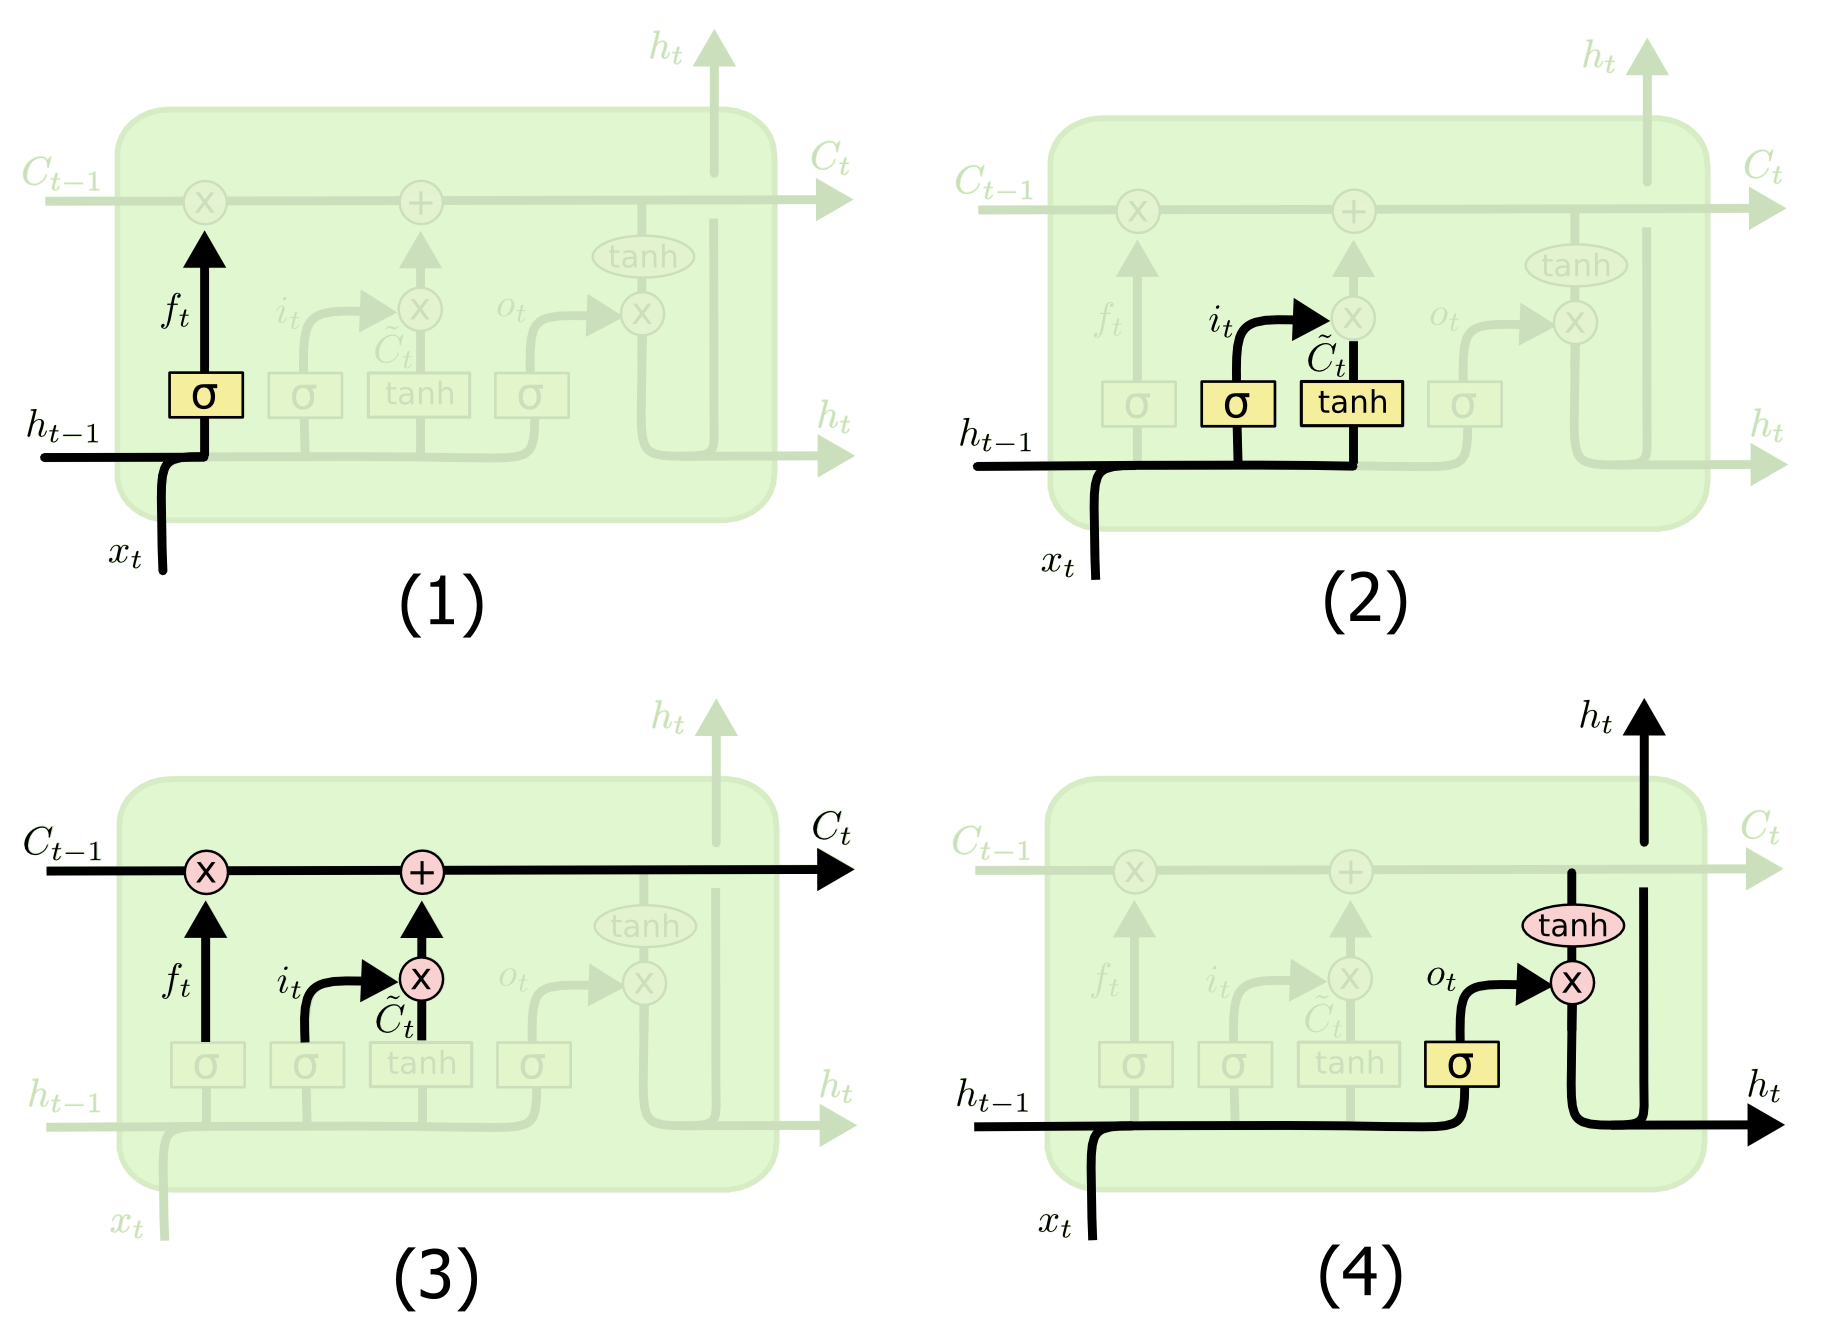
\includegraphics[height=3.5in]{Figures/LSTMs.png}
    \caption{ Recorrido por el funcionamiento de una celda LSTM. Figuras tomadas de \cite{olah}. }
    \label{LSTMrec}
  \end{center}
\end{figure}

En la figura \ref{LSTMrec}, se muestra el recorrido paso a paso del funcionamiento de una celda LSTM. 
El primer paso (panel 1) es decidir 
que parte de la información será descartada. Esta decisión se realiza por una sigmoide llamada en inglés ``\textit{forget gate layer}'':

\begin{equation}
  f_t = \sigma(W_f\cdot[h_{t-1},x_t]+b_f)
\end{equation}

Esta puerta recibe el input actual $x_t$ y la salida del tiempo anterior $h_{t-1}$ y arroja un valor entre 0 y 1, 0 significa
 `` olvidar esto completamente''  y 1 significa ``mantener esto completamente''. 

 El siguiente paso  (paneles 2 y 3)  se encarga de actualizar el estado de la celda del valor 
 de $C_{t-1}$ al nuevo valor $C_{t}$ y tiene dos partes, primero se multiplica el antiguo estado por $f_t$, y luego
 se suma el valor del nuevo candidato $C'_t$, escalado por un factor que cuantifica la magnitud del cambio:
 
 \begin{equation}
  C_t = f_t\cdot C_{t-1}+i_t\cdot C'_t
\end{equation}

donde,

 \begin{equation}
  i_t = \sigma(W_i\cdot[h_{t-1},x_t]+b_i)
\end{equation}

\begin{equation}
  C'_t = tanh(W_C\cdot[h_{t-1},x_t]+b_C)
\end{equation}



Finalmente, se calcula la salida $h_t$ de la siguiente manera (panel 4):

\begin{equation}
  o_t = \sigma(W_o\cdot[h_{t-1},x_t]+b_o)
\end{equation}

\begin{equation}
  h_t = o_{t}\cdot tanh(C_t)
\end{equation}

\section{Topología de los modelos utilizados}
Se han considerados 3 modelos que poseen una estructura básica que consta de una capa de entrada, dos o tres capas ocultas
y una capa de salida:


\begin{enumerate}
    \item \textbf{Modelo Denso}: En primer lugar se ha considerado un modelo que consta de dos capas densas, 
    en la figura \ref{Red_densa} podemos  ver  un resumen con las principales características de las mismas.
    \item \textbf{Modelo LSTM1}: En segundo lugar se ha considerado un modelo que contiene una capa LSTM y 
    una segunda capa densa (Fig. \ref{Red_LSTM1}).
    \item \textbf{Modelo LSTM2}: Por último se ha considerado un tercer modelo que consta de dos capas LSTM y una capa densa (Fig. \ref{Red_LSTM2}) que se 
    ha entrenado de manera secuencial.
    
    % utilizando únicamente los valores simulados de los caudales en la matriz $Y_{indv,id}$.
    % En este enfoque la red utiliza los valores de los caudales en tiempos anteriores
    %  $q_{t-1}, q_{t-2}, q_{t-n}$ para predecir el valor actual $q_{t}$. 
    %  La variable $n$ también llamada "look back" se puede elegir arbitrariamente y se puede ajustar haciendo 
    %  una busca con el método de cross validation.
\end{enumerate}

\begin{figure}[h!]
    \begin{center}
      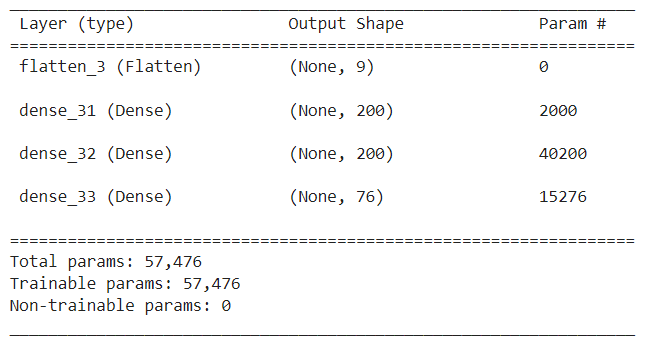
\includegraphics[height=2.in]{Figures/Red_densa.PNG}
      \caption{ Modelo Denso.}
      \label{Red_densa}
    \end{center}
  \end{figure}


  \begin{figure}[h!]
      \begin{center}
        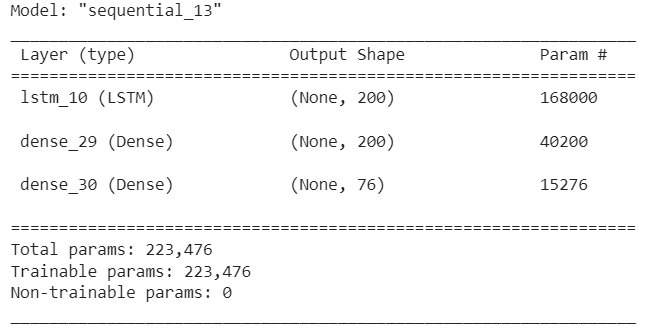
\includegraphics[height=2.in]{Figures/Red_LSTM.PNG}
        \caption{ Modelo LSTM1.}
        \label{Red_LSTM1}
      \end{center}
    \end{figure}
  
    \begin{figure}[h!]
        \begin{center}
          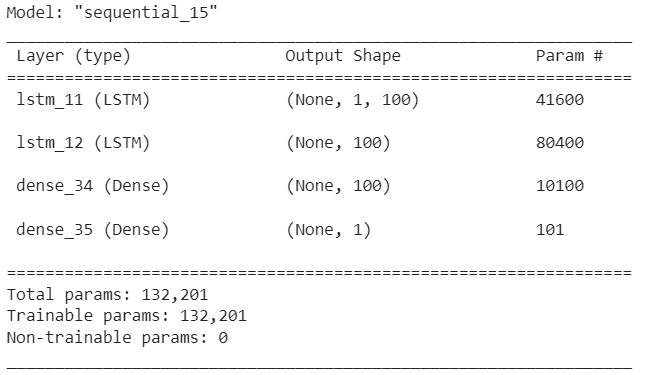
\includegraphics[height=2.1in]{Figures/Red_LSTM2.PNG}
          \caption{ Modelo LSTM2.}
          \label{Red_LSTM2}
        \end{center}
      \end{figure}
    
    

     
     

% \subsection{Modelo Denso}
% En primer lugar se ha considerado un modelo que consta de dos capas densas, en la figura \ref{Red_densa} podemos 
% ver  un resumen con las principales características de las mismas.
% \vspace{5mm}

% \begin{figure}[h!]
%     \begin{center}
%       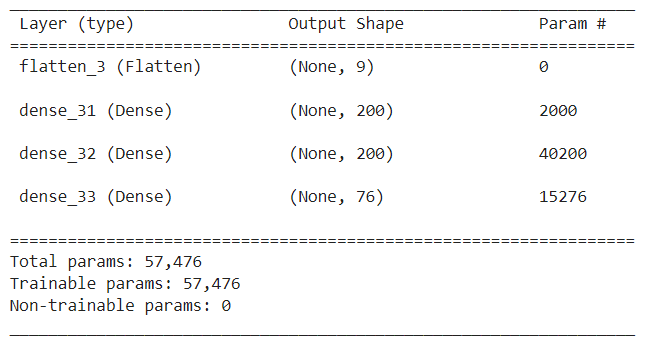
\includegraphics[height=2.in]{Figures/Red_densa.PNG}
%       \caption{ Modelo Denso}
%       \label{Red_densa}
%     \end{center}
%   \end{figure}


% \subsection{Modelo LSTM1}

% En segundo lugar se ha considerado un modelo que contiene una capa compuesta de una red recurrente y una segunda capa densa (Fig. \ref{Red_LSTM1})
% Se han utilizado dos maneras diferentes de entrenar este modelo, por un lado se ha entrenado sobre toda la cuenca,
% de la misma manera que el modelo denso, es decir utilizando las matrices $X_{comp}$ e $Y_{comp}$, 
% \begin{figure}[h!]
%     \begin{center}
%       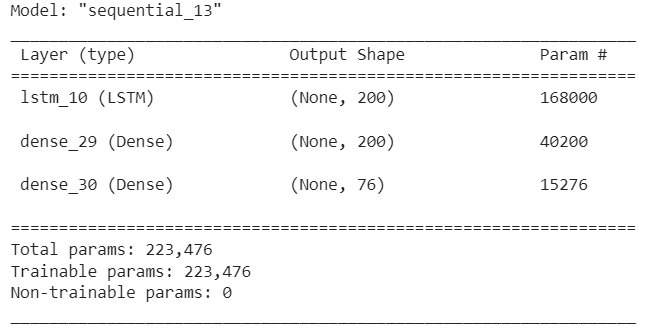
\includegraphics[height=2.in]{Figures/Red_LSTM.PNG}
%       \caption{ Modelo LSTM 1 }
%       \label{Red_LSTM1}
%     \end{center}
%   \end{figure}

%   \vspace{5mm}

% \subsection{Modelo LSTM2}

% \begin{figure}[h!]
%     \begin{center}
%       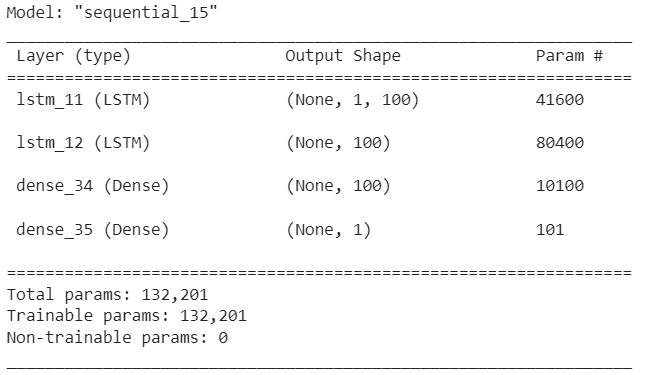
\includegraphics[height=2.in]{Figures/Red_LSTM2.PNG}
%       \caption{ Modelo LSTM 2}
%       \label{Red_LSTM2}
%     \end{center}
%   \end{figure}


% Por último se ha considerado un tercer modelo que consta de dos capas LSTM y una capa densa (Fig. \ref{Red_LSTM2}).




\subsection{Regularización de la función de coste}
Se han considerado dos tipos de regularizaciones, L1 y L2 que penalizan el loss añadiendo
los siguientes términos para cada caso:

\begin{equation}
    loss + \lambda \sum |\omega_i| ~~(L1)
\end{equation}

\begin{equation}
    loss + \lambda \sum \omega^2_i ~~(L2)
\end{equation}

La función de estos términos extra es la de reducir el valor de los parámetros haciendo incluso que la influencia de 
algunas variables de entrada sea nula en la salida de la red, lo que da lugar a una selección de variables de forma natural y
reduce el posible sobreajuste de los datos. El valor de $\lambda$ varía entre 0 y 1 y controla la magnitud
de la reducción de los parámetros. 


\subsection{Funciones de activación}
En todas las capas se ha considerado la misma función de activación $f$, y se han entrenado los modelos considerando 
las opciones mostradas en \ref{activation}.

\begin{table}[h!]
    \centering
    \begin{tabular}{|c|c|}   
        \hline
        &\\
     $ f(x)= \frac{1}{e^{-x}+1}$ ~(sigmoide) & 
     $f(x) = \left\lbrace
     \begin{array}{ll}
     0 &\textup{si } x\leq 0 \\
     x & \textup{si } x > 0 
     \end{array}
     \right. ~(relu)$    \\
     &\\
     \hline
     &\\
     $f(x)= \frac{e^{2x}-1}{e^{2x}+1} ~(tanh)$ & $f(x)=x ~ (linear)$    \\ 
     &\\
     \hline
    \end{tabular}
    \caption{ Funciones de activación}
    \label{activation}
    \end{table}


\subsection{Optimizadores}

\begin{figure}[h!]
  \begin{center}
    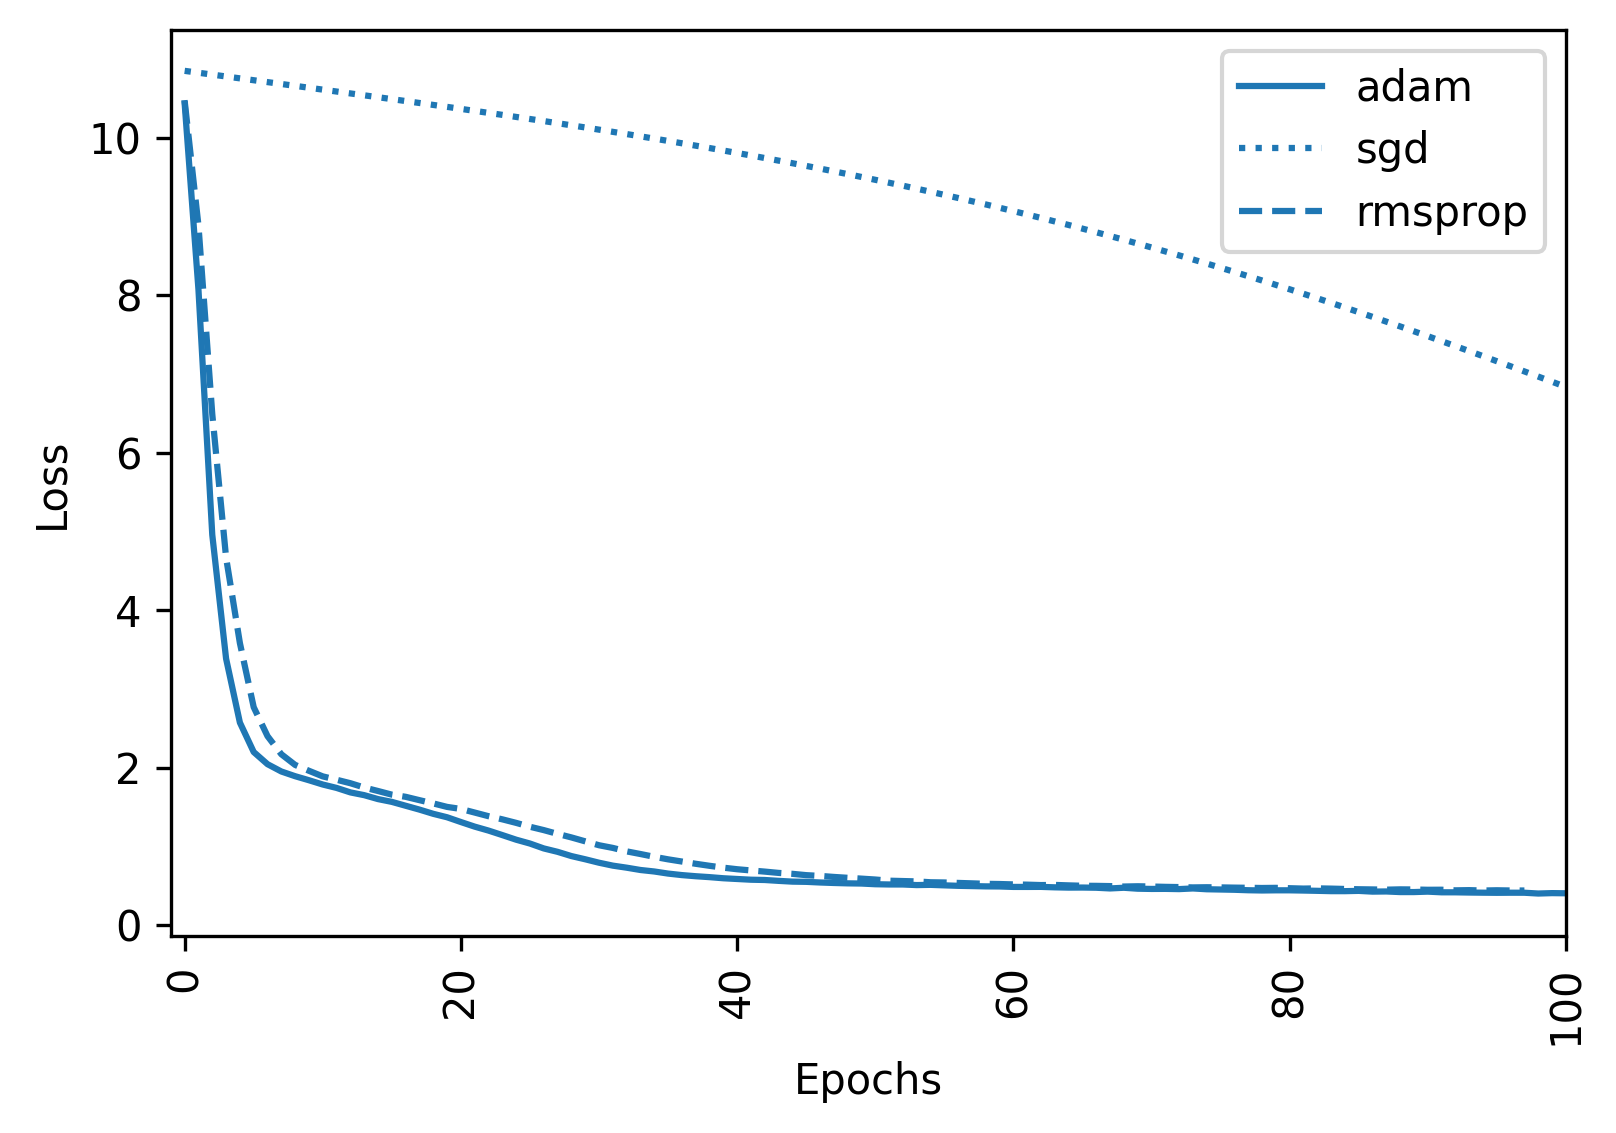
\includegraphics[height=3.in]{Figures/optims.png}
    \caption{ Evolución de la función de loss considerando diferentes optimizadores.}
    \label{opt}
  \end{center}
\end{figure}

Dado el gran número de diferentes pesos y observaciones, el cálculo de la derivada parcial de la función de coste 
respecto a cada uno de los pesos de la red para cada observación es inviable. Existen diferentes métodos que optimización
este proceso y agilizan los cálculos. En este trabajo se ha hecho una exploración inicial manual para evaluar 
la performance de los optimizadores 
"\textit{Stochastic Gradient Descent}" (SGD) \cite{optim}, "\textit{Adaptive moment estimation}" (Adam) \cite{adam} y 
\textit{Root Mean Square Propagation} (RMSprop) \cite{optim}.



En la figura \ref{opt} se muestra a modo de ejemplo la evolución de la función de loss considerando cada uno de los 
optimizadores al entrenar el modelo LSTM1, se puede ver que la taza de aprendizaje con adam y rmspror es considerablemente
mayor que con sgd, ya que en los primeros casos la función de loss alcanza su valor de equilibrio en aproximadamente 
60 épocas, mientras que sgd necesita más de 200. 



\subsection{Calibración de los modelos}
\label{cal}

\begin{figure}[h!]
  \begin{center}
    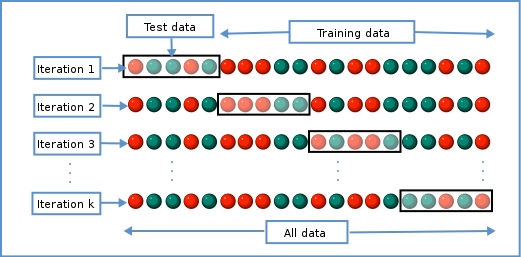
\includegraphics[height=2.in]{Figures/GridsearchCV.png}
    \caption{ k-fold cross validation (imagen de Gufosowa - WikiMedia).}
    \label{KCV}
  \end{center}
\end{figure}


Los modelos se calibran realizando una búsqueda exhaustiva de hyper-parámetros utilizando el 
con el método "GridSearchCV" disponible en la librería scikit-learn \cite{scikit}.
Éste método crea una grilla con los hyper-parámetros del modelo y optimiza sus valores realizando una búsqueda
 con validación cruzada, en donde el conjunto de datos se divide en datos de entrenamiento y de validación 
 (train/test en la figura \ref{KCV}).  Cómo este conjunto se divide y cuantas veces se realiza el proceso, se controla mediante el 
 número de pliegues o folds, en general denotado con la letra k.
 El modelo utiliza el primer fold en la primera iteración como conjunto de test y 
 los siguientes k-1 como conjunto de train. Este proceso se repite k veces para cada uno de las posibles 
 combinaciones de hyper-parámetros presentes en la grilla y arroja como resultado final un valor promedio 
 del escore utilizado para evaluar  la calidad del modelo. 

 \begin{table}[h!]
  \begin{center} 
  \begin{tabular}{|l|l|l|}
    \hline
   Modelo&Parámetros &  valores \\
   \hline
   &solver &  rmsprop, adam, sgd\\
   &Neuronas &  10, 80, 200 \\
   Denso &activación & sigmoid,relu,tanh,linear \\
   &alpha &  0.0001,0.0002,0.0003 \\
   &Regularización & l1,l2 $\lambda = 0.0001,0.001,0.1$  \\
   \hline
   &solver &   rmsprop, adam, sgd\\
   &Neuronas &  10, 80, 200 \\
   LSTM1 PCA &activación & sigmoid,relu,tanh,linear \\
   &alpha &  0.0001,0.0002,0.0003 \\
   &Regularización & l1,l2 $\lambda =0.0001,0.001,0.1$  \\

   \hline
   &solver &   rmsprop, adam, sgd\\
   &Neuronas &  10, 80, 200 \\
   LSTM1 loc &activación & sigmoid,relu,tanh,linear \\
   &alpha &  0.0001,0.0002,0.0003 \\
   &Regularización & l1,l2 $\lambda =0.0001$  \\

   \hline
   &solver &   rmsprop, adam, sgd\\
   &Neuronas &  10, 80, 200 \\
   LSTM2 &activación & sigmoid,relu,tanh,linear \\
   &alpha & 0.001 \\
   &Regularización & l1,l2 $\lambda =0.0000001$  \\
   \hline

  \end{tabular}
  \caption{ Hyper parámetros explorados en los diferentes modelos.}
  \label{hyper}
\end{center}
  \end{table}


  En la tabla \ref{hyper} se muestran los hyper-parámetros explorados para entrenar los diferentes modelos. En el caso
  del entrenamiento global, realizado para los modelos denso y LSTM1 PCA, tres de 
  estos parámetros (el número de neuronas, la función de activación y $\lambda$) 
  han sido optimizados mediante el método GridSearchCV.


  \section{Entrenamiento}
  Los modelos han sido entrenados durante un número de épocas o pasos
  igual a 200 y se ha utilizado el callback "\textit{early stopping}" con paciencia 3, 
  que interrumpe la ejecución cuando el valor del loss en el conjunto de validación aumenta durante tres iteraciones sucesivas. 
Se han considerado tres métodos diferentes de entrenamiento que se describen a continuación.

% \begin{itemize}
%     \item Entrenamiento global, considerando las series hidro-climáticas de entrada de la cuenca en su totalidad 
%     \item Entrenamiento local,  considerando las series hidro-climáticas de entrada locales para cada sub-cuenca.
%     \item Secuencial, considerando los datos de las series temporales de salida de manera secuencial.
% \end{itemize}en primer lugar se han entrenado los 
 
  \subsection{Entrenamiento global}
 Los modelos denso y LSTM1 han sido entrenados sobre una matriz que contiene las entradas o variables características 
 (series temporales de precipitación, temperatura máxima y temperatura mínima) para 
todas las subcuencas que constituyen la cuenca hidrológica Chambo:
  
  \vspace{5mm}
  
    \begin{equation*}
      X_{comp}= 
      \begin{bmatrix}
          p_{1,1} & T^{max}_{1,1} &  T^{min}_{1,1}& p_{1,2} & T^{max}_{1,2} &  T^{min}_{1,2} & ... &p_{1,nc} & T^{max}_{1,nc} &  T^{min}_{1,nc} \\
          ... & ... &  ...& ... & ...&  ... & ... &... & ... &  ... \\
          p_{nt,1} & T^{max}_{nt,1} &  T^{min}_{nt,1}& p_{nt,2} & T^{max}_{nt,2} &  T^{min}_{nt,2} & ... &p_{nt,n} & T^{max}_{nt,n} &  T^{min}_{nt,nc} \\
          \end{bmatrix}
  \end{equation*}
  
  \vspace{5mm}
  
  
  Donde $n_t$ es el número de pasos temporales y $nc$ es el número de subcuencas. 
  Las variables objetivo son los caudales naturales simulados con el modelo hidrológico LEM y 
  se encuentran almacenados en una matriz $Y_{comp}$ estructurada de la siguiente manera:
  
  \vspace{5mm}
  
  \begin{equation*}
      Y_{comp}= 
      \begin{bmatrix}
          q_{1,1} & q_{1,2} & q_{1,2} ... &  q_{1,nc} \\
          ... & ... & ... &  ... \\
          q_{nt,1} & q_{nt,2} & q_{nt,2} ... &  q_{nt,nc} \\
          \end{bmatrix}
  \end{equation*}
  
  \vspace{5mm}
  
  El paso  de tiempo que se ha considerado es mensual y el rango temporal total es de 20 años 
  (desde el año 2000 hasta el año 2020). Por otro lado la cuenca se encuentra compuesta por 76 subcuencas, 
  entonces las dimensiones de $X_{comp}$ e $Y_{comp}$ son (229,228) y (229,76), respectivamente.
  Finalmente, los datos han sido divididos en conjuntos de train y test tomando los primeros 160 
  como conjunto de train y los últimos 69 como conjunto de test.

  Para el caso de capas LSTM es necesario agregar una dimensión a las matrices de entrada que toma en cuenta la correlación temporal de las muestras. 
  La estructura de las matrices de entrada toman la forma (\textit{muestras}, \textit{pasos de tiempo}, \textit{características}). En el modelo 
  LSTM1 se considera un paso de tiempo por cada muestra, por lo cual  las matrices toman 
  la dimensión (229,1,228) y (229,1,76), respectivamente.

\subsection{Entrenamiento local}
 Por otro lado el modelo LSTM1 también se ha entrenado individualmente cuenca por cuenca, para lo cual se han utilizado
matrices $X_{loc}$ e $Y_{loc}$ con las siguientes formas:
\vspace{5mm}

\begin{equation*}
    X_{loc,id}= 
    \begin{bmatrix}
        p_{1,id} & T^{max}_{1,id} &  T^{min}_{1,id} \\
        ... & ... &  ... \\
        p_{nt,id} & T^{max}_{nt,id} &  T^{min}_{nt,id} \\
        \end{bmatrix}
\end{equation*}

\vspace{5mm}


\begin{equation*}
    Y_{loc,id}= 
    \begin{bmatrix}
        q_{1,id}  \\
        ...  \\
        q_{nt,id}  \\
        \end{bmatrix}
\end{equation*}

\vspace{5mm}

Donde $id$ es el número de la subcuenca. 
\vspace{5mm}

En este último caso, las matrices poseen las dimensiones (229,1,3) y (229,1,1), respectivamente. 
La división entre los conjuntos de entrenamiento y test se ha hecho de la misma manera que en el apartado anterior.

\subsection{Entrenamiento secuencial}

Finalmente, el modelo LSTM2 se ha entrenado de manera secuencial, utilizando únicamente los valores simulados de los caudales 
en la matriz $Y_{loc,id}$. En este enfoque, la red utiliza los valores de los caudales en tiempos anteriores
 $q_{t-1}, q_{t-2}, q_{t-n}$ para predecir el valor actual $q_{t}$. 
 La variable $n$ también llamada "look back" se puede elegir arbitrariamente y se puede ajustar haciendo 
 una busca con el método de cross-validation.


\section{Análisis de componentes principales}

El espacio de variables predictoras del conjunto de entrenamiento 
que contiene la información de las 76 subcuencas posee una dimensión (160,228).
Sin embargo, existen correlaciones entre las variables que 
provocan que muchas de estas aporten información poco relevante o redundante \cite{Manu}. 
Estas correlaciones pueden distorsionar el proceso de aprendizaje de los modelos \cite{gutierrez} 
y es por eso que se ha optado por reducir el número de variables mediante el análisis de componentes principales\cite{PCA}.

Este método realiza una transformación del espacio predictor a un espacio vectorial 
cuya base son los auto-vectores de la matriz de covariancia. 
En este espacio, los valores en la diagonal de dicha matriz son las varianzas
en la dirección de cada uno de los vectores de la base o componentes principales.
La reducción de dimensiones se realiza escogiendo las direcciones que captan la mayor variación 
de los datos originales, es decir las PCA con las mayores varianzas. 

Luego de realizar este análisis se ha encontrado que se puede explicar el 96$\%$ de la varianza del conjunto
de datos original considerando sólo las primeras 9 componentes (ver figura \ref{PCA}). Por lo tanto la reducción del espacio
predictor es considerable, ya que ha pasado de ser (160,228) a (160,9).

\begin{figure}[h!]
  \begin{center}
    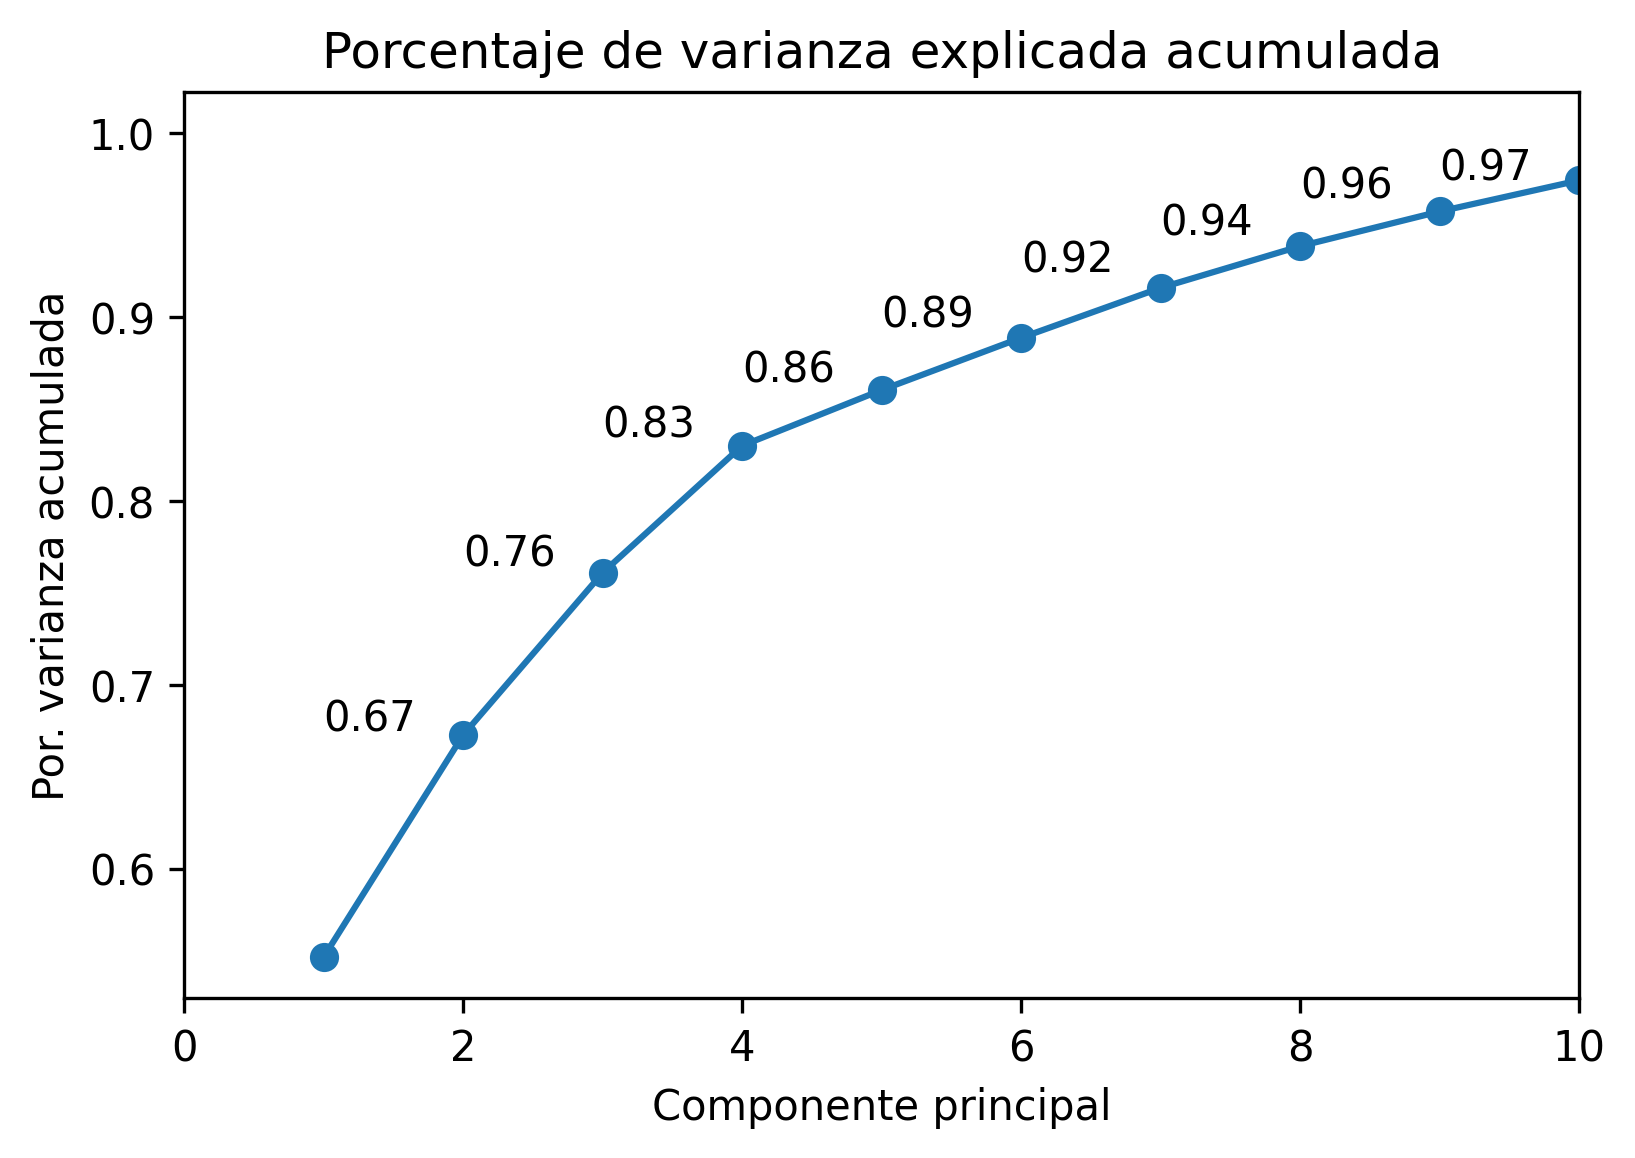
\includegraphics[height=2.5in]{Figures/PCA.png}
    \caption{ Porcentaje de varianza explicada acumulada para las primeras 9 componentes principales.}
    \label{KCV}
  \end{center}
\end{figure}

\section{Coeficiente de Nash-Sutcliffe}
\label{sectNSE}


\begin{table}[h!]
  \begin{center}
  \begin{tabular}{|c|c|}
    \hline
    Calidad del ajuste &   NSE  \\
    \hline
     &   \\
   Excelente & $0.75 < NSE \leq 1.00$   \\
   Bueno &  $0.65<  NSE \leq 0.75$ \\
   Aceptable &  $0.5<  NSE \leq 0.65$  \\
   No aceptable &  $ NSE \leq 0.5$ \\
   &   \\
   \hline
  \end{tabular}
  \caption{Calidad de los ajustes en función del coeficiente NSE \cite{NSE}.}
  \label{tablaNSE}
\end{center}
  \end{table}

Además de utilizar la función de loss para validar los modelos durante el entrenamiento, 
también se ha utilizado el coeficiente Nash-Sutcliffe (NSE) \cite{NSE} para evaluar la performance de los mismos en el conjunto de test. 
Este coeficiente es uno de los más utilizados en hidrología y se define de la siguiente manera:

\begin{equation}
  NSE = 1-\frac{\sum^n_i(y_i-\hat{y}_i)^2}{\sum^n_i(\bar{y}-\hat{y}_i)^2}
\end{equation}

Los valores de NSE varían entre $-\infty$ y 1, siendo este último valor el correspondiente a un ajuste perfecto.
En la tabla \ref{tablaNSE} se indica la relación entre los valores de NSE y la calidad de los ajustes.
Este coeficiente equivale a una combinación lineal del error medio
cuadrático, la desviación y el coeficiente de correlación
entre las series.


%  \subsection{Validación de los modelos}

%  \begin{figure}[h!]
%    \begin{center}
%      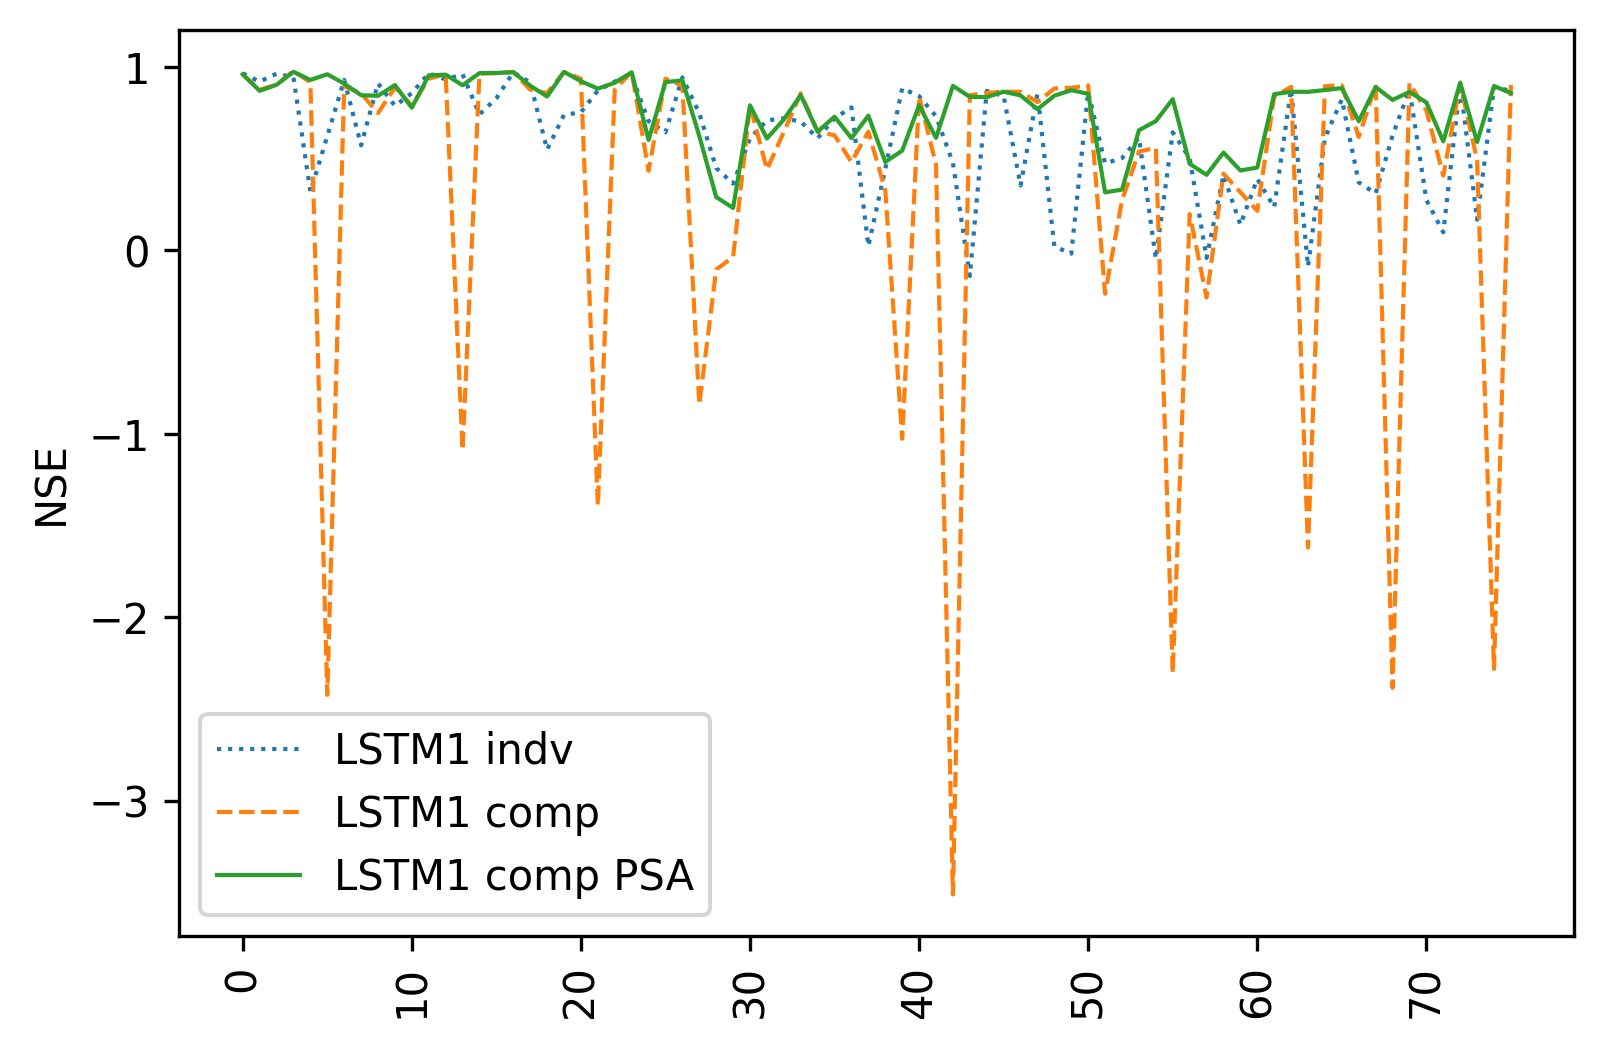
\includegraphics[height=3.in]{Figures/NSEs_1.png}
%      \caption{ Modelo LSTM 2}
%      \label{NSE1}
%    \end{center}
%  \end{figure}

% Para validar los modelos y hacer un análisis un poco más profundo de cómo es su performance en los diferentes puntos
% de la cuenca, se ha utilizado el coeficiente de Nash-Sutcliffe (NSE). En la figura \ref{NSE1} se muestran los valores obtenidos 
% de NSE en todas las subcuencas para el modelos LSTM1. La curva punteada muestra los valores obtenidos al entrenar el modelo en 
% cada subcuenca de forma individual, la curva dashed es la obtenida entrenando el modelo para toda la cuenca en conjunto
% considerando la matriz$X_{comp}$ que posee 288 características. Se puede observar que para este modelo, 
% el valor de NSE baja considerablemente en muchos puntos, esto se debe a que al haber tantas características 
% de entrada se produce un sobre ajuste de los datos. Esto se puede corregir haciendo una reducción del espacio considerando
% las componente principales (curva sólida). En este análisis el número de características se reduce a 9 componentes principales 
% que explican el $96\%$ de la varianza de los datos.

% %   \begin{figure}[h!]
% %     \begin{center}
% %       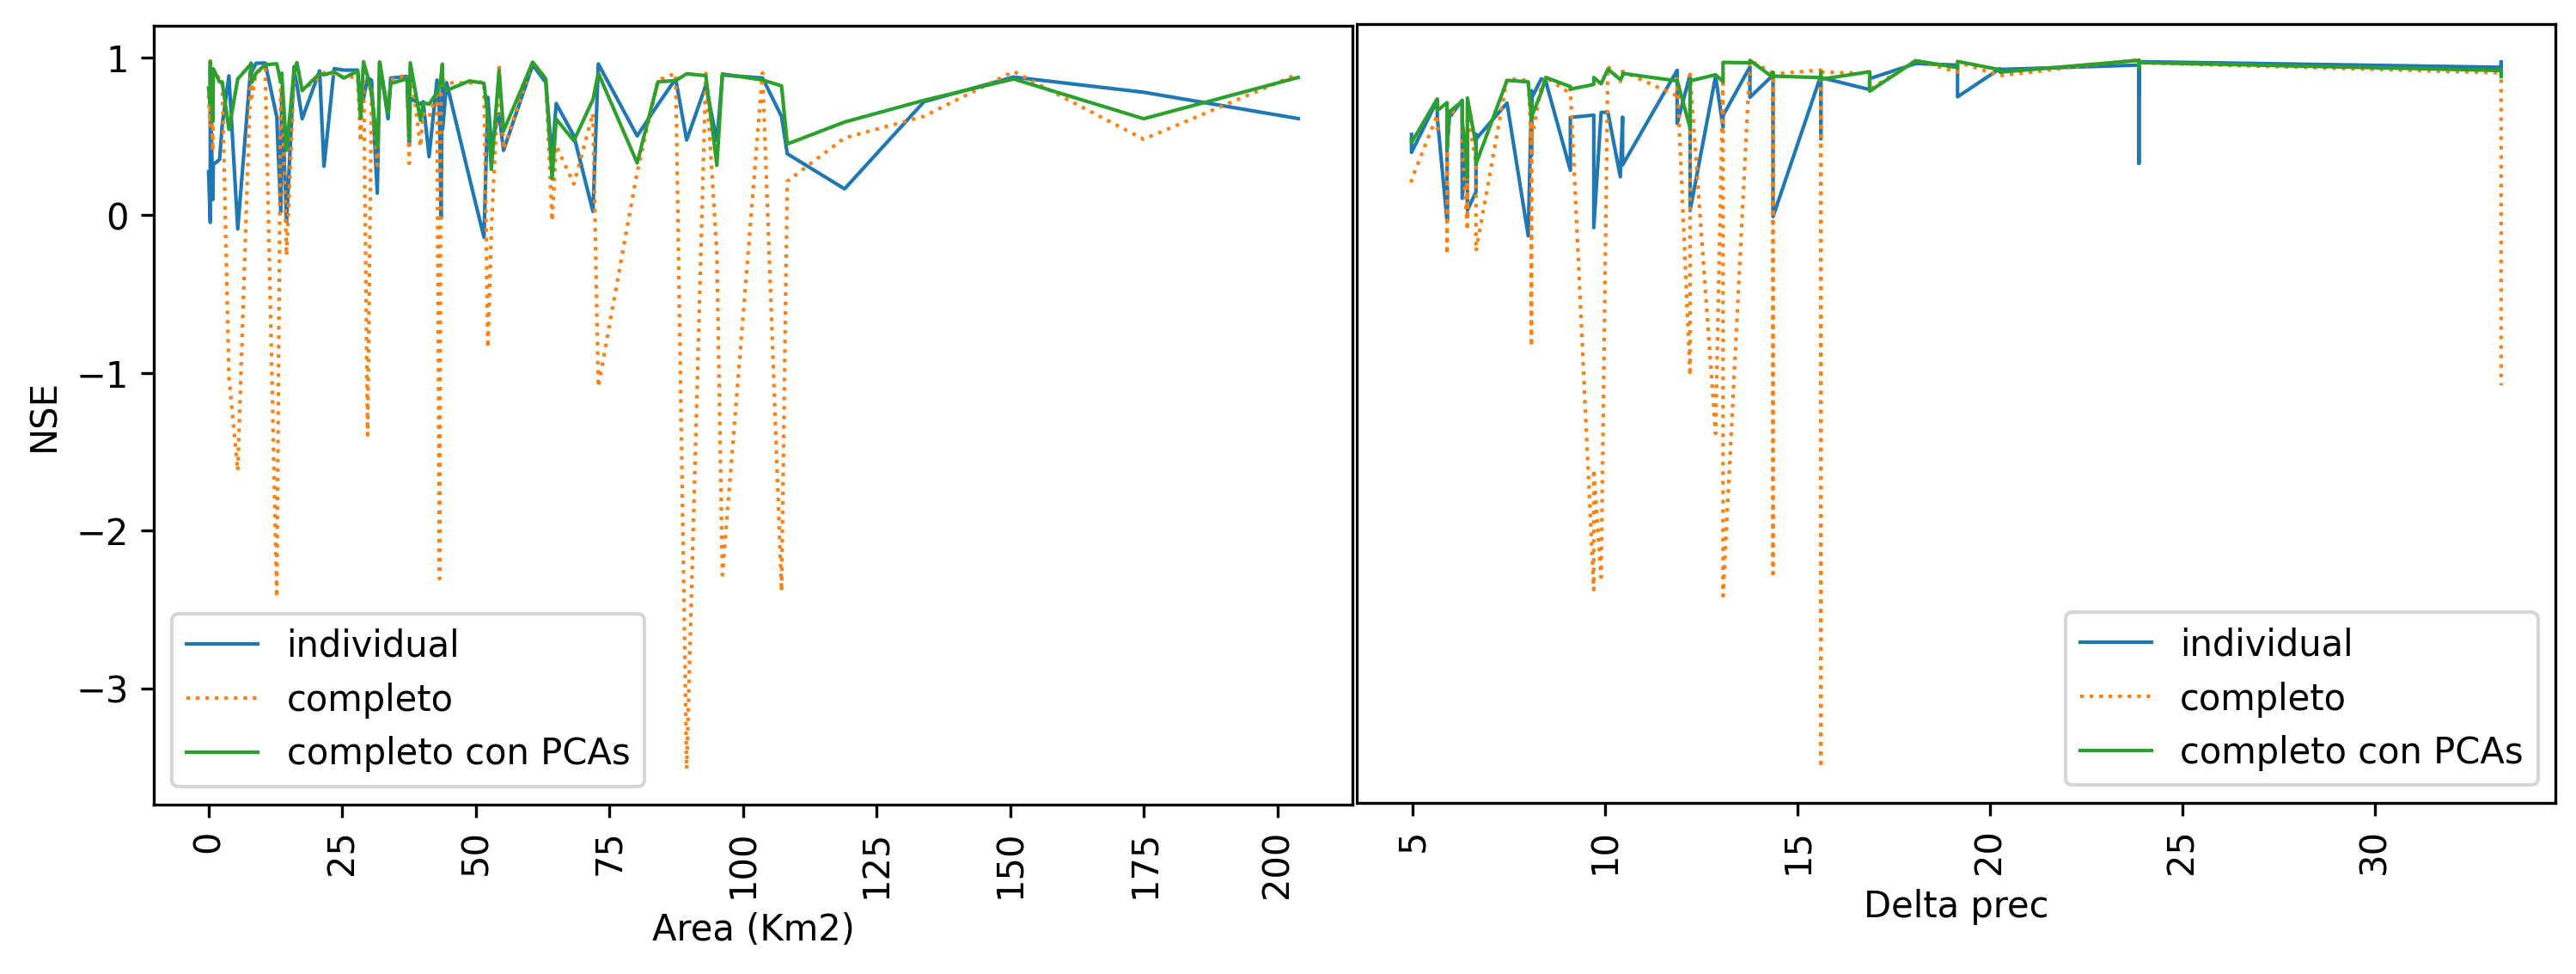
\includegraphics[height=2.3in]{Figures/NSEs_Area_prec.png}
% %       \caption{ Modelo LSTM 2}
% %       \label{NSEs_Area_prec}
% %     \end{center}
% %   \end{figure}

%    \begin{figure}
%    \centering
%    \begin{subfigure}[b]{1\textwidth}
%        \centering
%        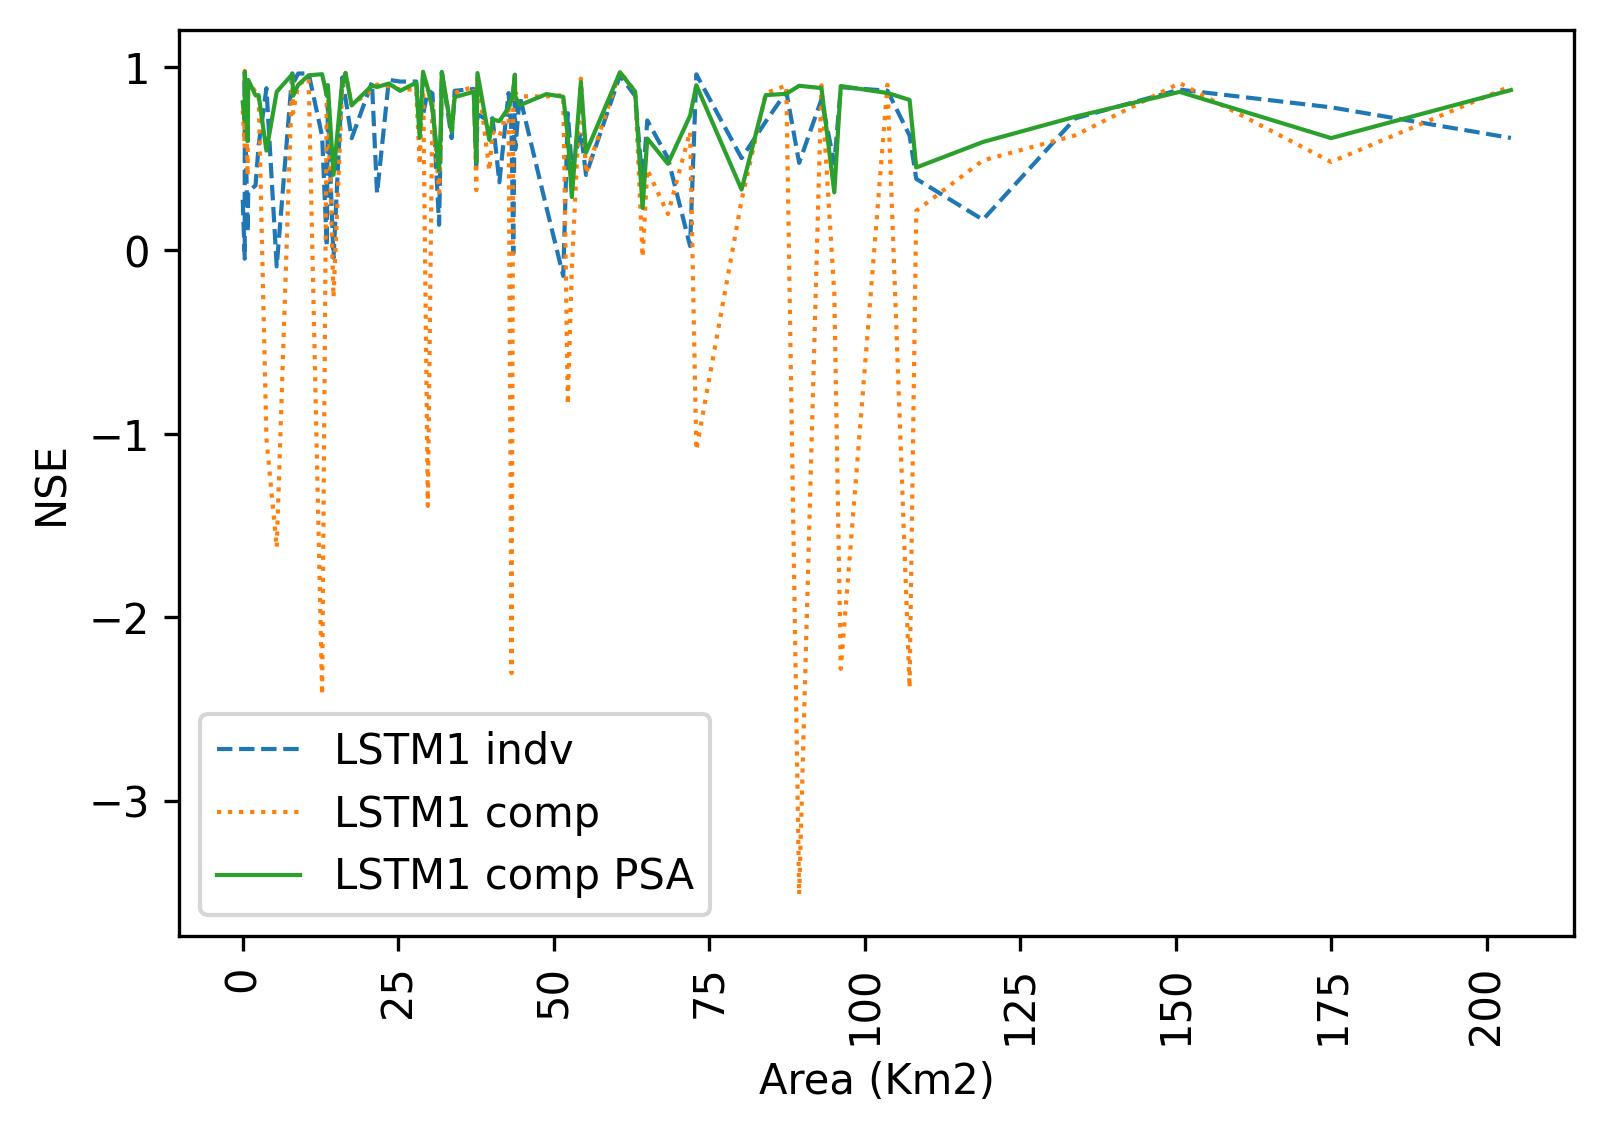
\includegraphics[width=\textwidth]{Figures/NSEs_Area.png}
%        \caption{}
%        \label{area}
%    \end{subfigure}
%    \hfill
%    \begin{subfigure}[b]{1\textwidth}
%        \centering
%        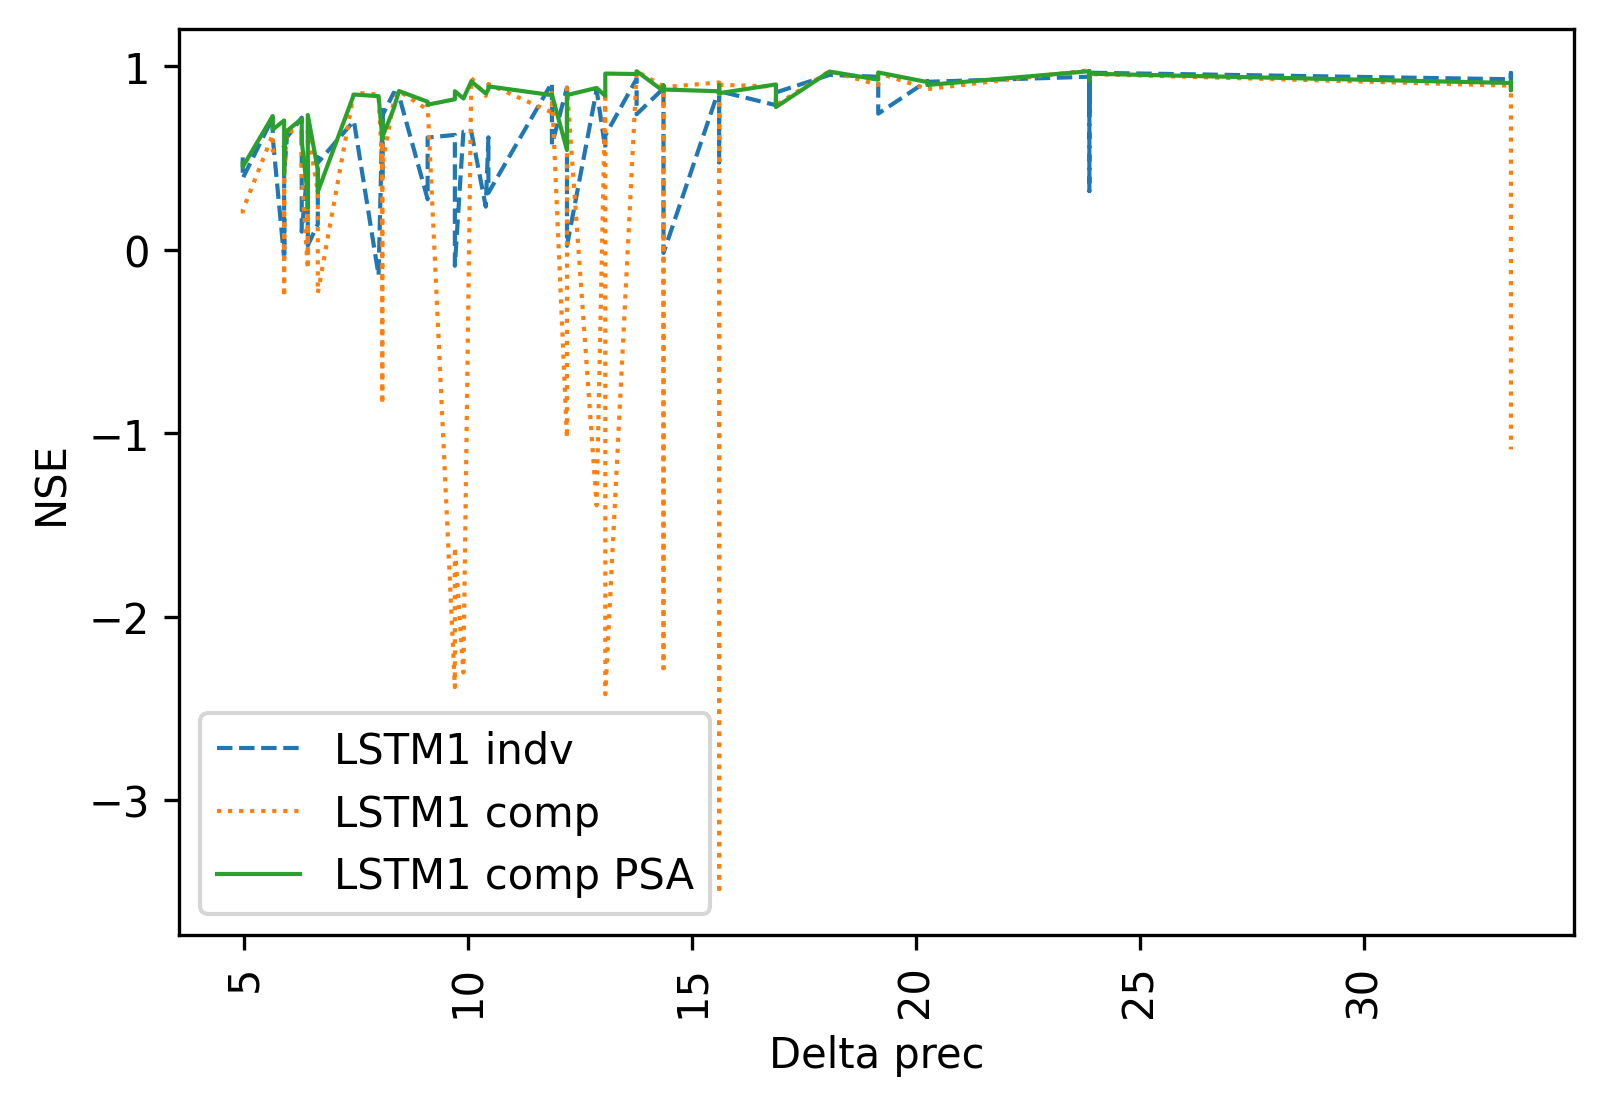
\includegraphics[width=\textwidth]{Figures/NSEs_Delta prec.png}
%        \caption{}
%        \label{Dp}
%    \end{subfigure}
%       \caption{Coeficientes de Nash-Sutcliffe en función del área (\ref{area}) y la variación de presión (\ref{Dp}).}
%       \label{NSEs_Area_prec}
% \end{figure}



%  Con el fin de determinar si hay otros factores que provocan el sobre ajuste de los datos,
%  en la figura \ref{NSEs_Area_prec} se muestran los valores de NSE en función del área de las cuencas (panel izquierdo) y 
%  de   la variación máxima de precipitación (panel derecho). Se puede observar que los modelos tienden a fallar 
%  para cuencas con áreas pequeñas ($A<125~km^2$) y cuando la serie de precipitación no muestra grandes variaciones 
%  ($\Delta P < 20~mm/d$). Esto se debe a que en este caso es difícil para los modelos poder distinguir los verdaderos patrones 
%  de precipitación del ruido, una alternativa para mejorar estos resultados sería considerar una capa de autoencoder al 
%  inicio de los modelos que permitan filtrar el ruido en los datos. 
 
%  Este efecto es aún más visible cuando entrenamos los modelos 
%  de manera local, si comparamos la curva continua con la dashed, podemos ver que en la mayoría de los casos, los resultados obtenidos
%  entrenando el modelo en toda la cuenca son mejores que cuando lo hacemos de manera individual. Esto se debe a que en el primer caso
%  estamos considerando  los patrones de precipitación en diferentes puntos de la cuenca, y aunque localmente 
%  la variación de la precipitación sea pequeña, la red aprende a completar la información faltante utilizando 
%  la información de toda la cuenca. En el segundo caso sólo  consideramos   los patrones locales en una cuenca dada y si la información
%  otorgada por la serie de precipitación no es buena (la variación es pequeña y no se reconoce un patrón claro) la red  
% no es capaz de completar la información necesaria con información proveniente de otros puntos de la cuenca. 

% * Agregar coeficiente NSE 
% * Agregar descripcion sobre la grilla de parametros con tabla y alguna graficas
% * Agregar lo de las PCAs

% \section{Resultados}
% * Agregar funciones de loss
% * Graficas de las distribuciones de los pesos? para ver que patrones se forman?

% \begin{figure}[h!]
%     \begin{center}
%       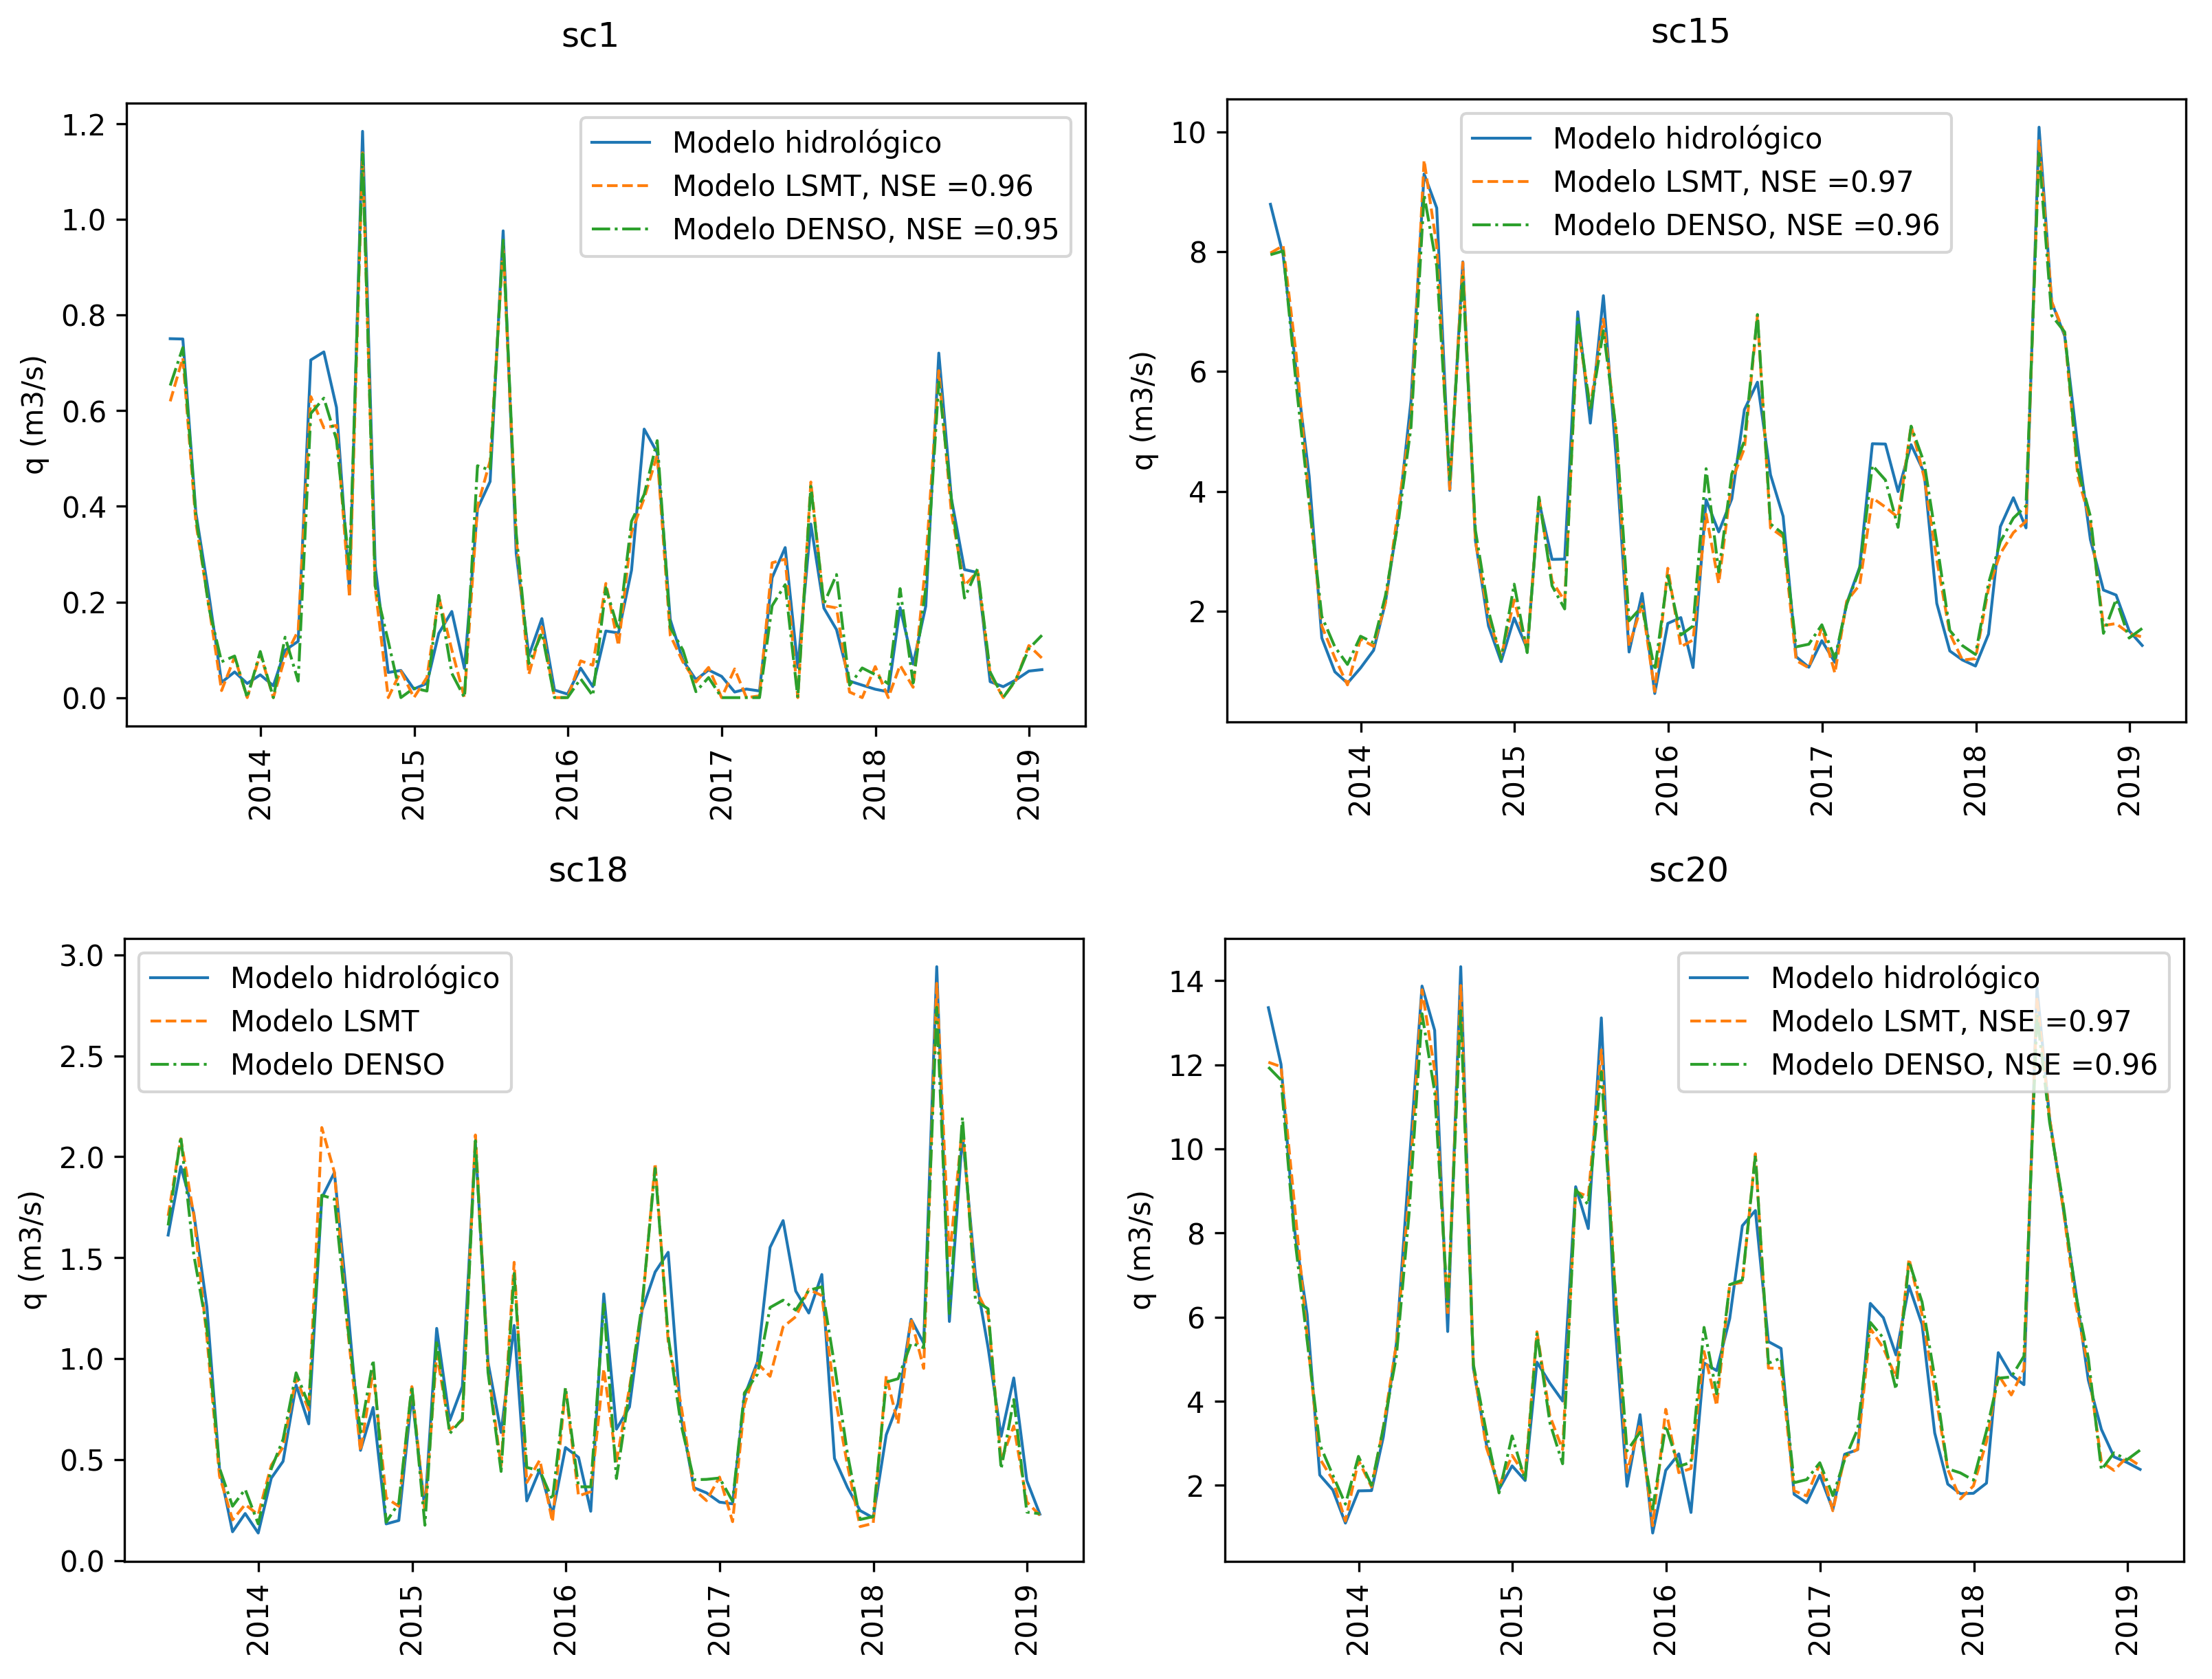
\includegraphics[height=4.in]{Figures/comparacion_scs.png}
%       \caption{ Resultados del Modelo LSTM 2.}
%       \label{autocorrelacion}
%     \end{center}
%   \end{figure}

% En la figura \ref{resultados_q} se muestran a modo de ejemplo los resultados obtenidos para los caudales de tres puntos
% diferentes de la cuenca, la sub-cuenca 1 , la sub-cuenca 20 y la 73 .
% En las figuras se muestran los resultados de los caudales simulados con el modelo hidrológico y los obtenidos con 
% los modelos Denso y LSTM1 en el conjunto de test. Se puede apreciar que agregar una capa LSTM mejora ligeramente los resultados
% ya que se incrementa el valor del coeficiente Nash-Sutcliffe (NSE) para el modelo. Esto era de esperar ya que la red LSTM
% tiene en consideración la dependencia temporal de las diferentes entradas mientras que el modelo denso considera las entradas
% de los distintos pasos de tiempo como independientes. 



% \begin{figure}[h!]
%     \begin{center}
%       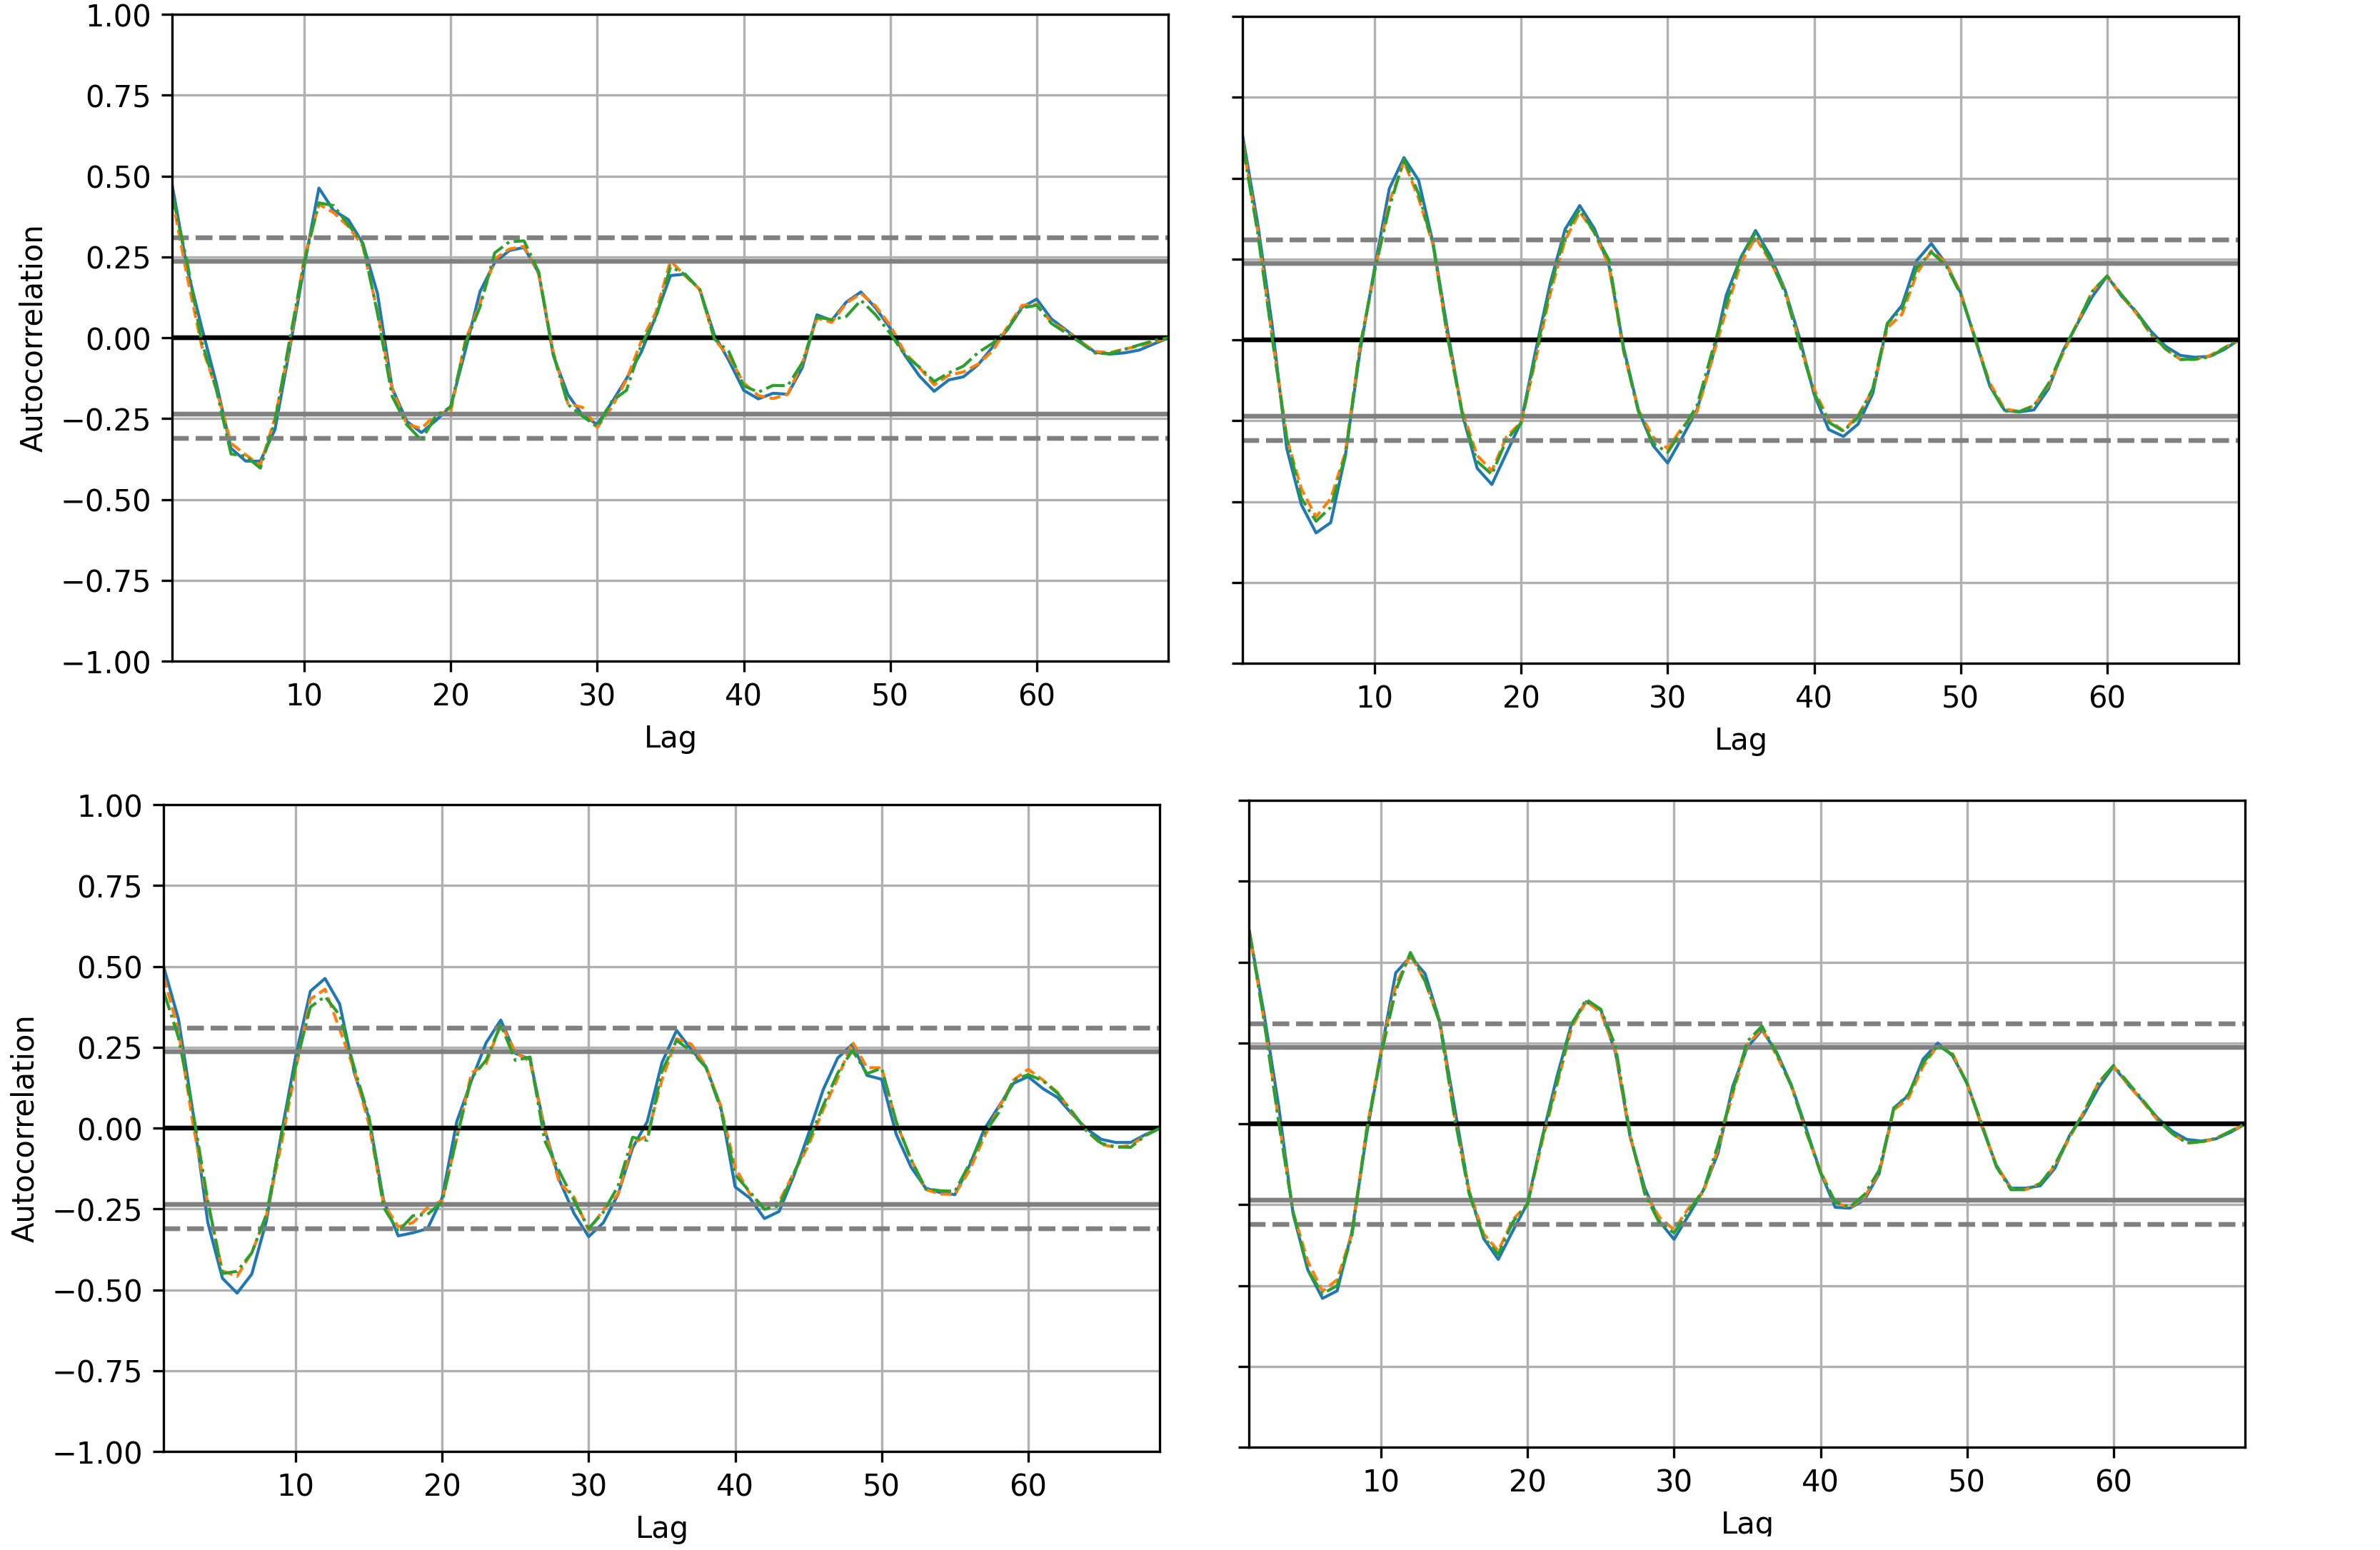
\includegraphics[height=3.5in]{Figures/autocorr_scs.png}
%       \caption{ Funciones de autocorrelación.}
%       \label{resultados_q}
%     \end{center}
%   \end{figure}

% En la figura \ref{autocorrelacion} se muestran las funciones de autocorrelación
% correspondientes a cada una de la subcuencas. Se puede observar que ambos modelos son capaces de captar correctamente 
% la estacionalidad de los datos.



%  \begin{figure}[h!]
%     \begin{center}
%       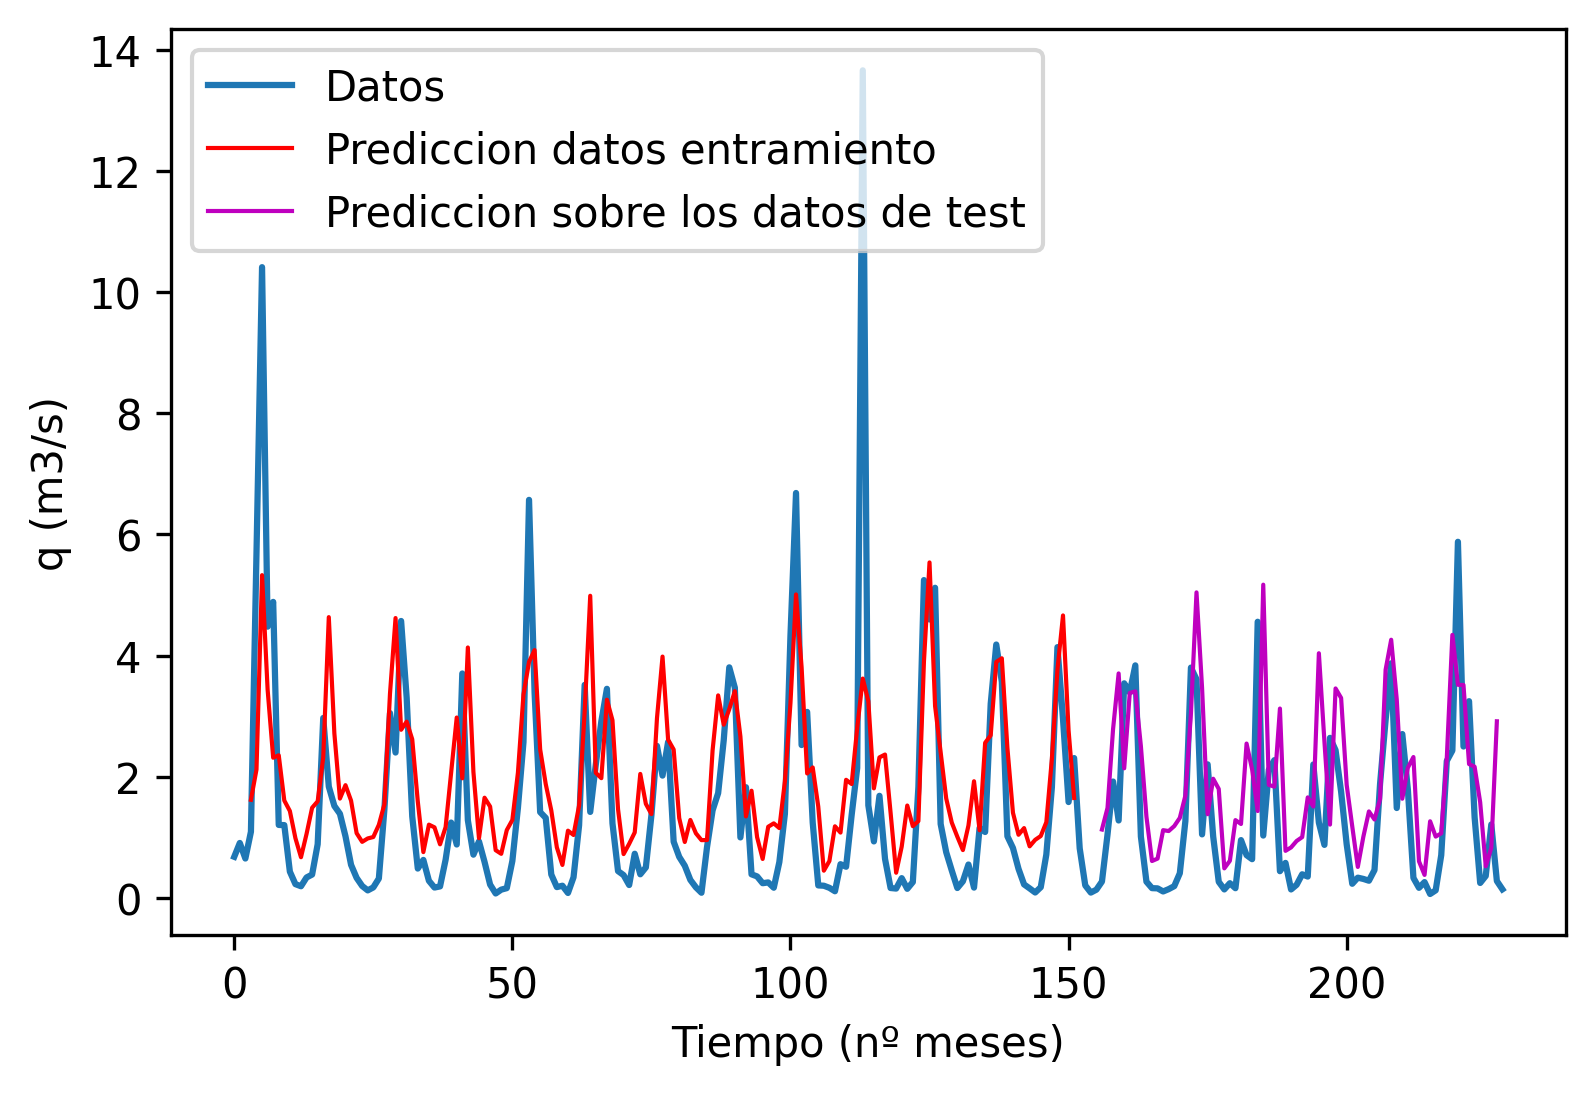
\includegraphics[height=3.in]{Figures/modelo_LSTM_seq.png}
%       \caption{ Resultados del modelo LSTM 3.}
%       \label{result_LSTM3}
%     \end{center}
%   \end{figure}


%   En la figura \ref{result_LSTM3} se muestran los resultados obtenidos con el modelo LSTM3 en todo el rango de datos 
%   para la subcuenca numero 73. En este enfoque, se han predicho los datos de manera secuencial, 
%   para lo cual sólo se ha utilizado la información de las series temporales de los caudales simulados en el
%   conjunto de entrenamiento. Si bien este modelo predice   correctamente la tendencia de los datos, 
%   falla al predecir los valores de los caudales.

  





% %   \begin{figure}[h!]
% %     \begin{center}
% %       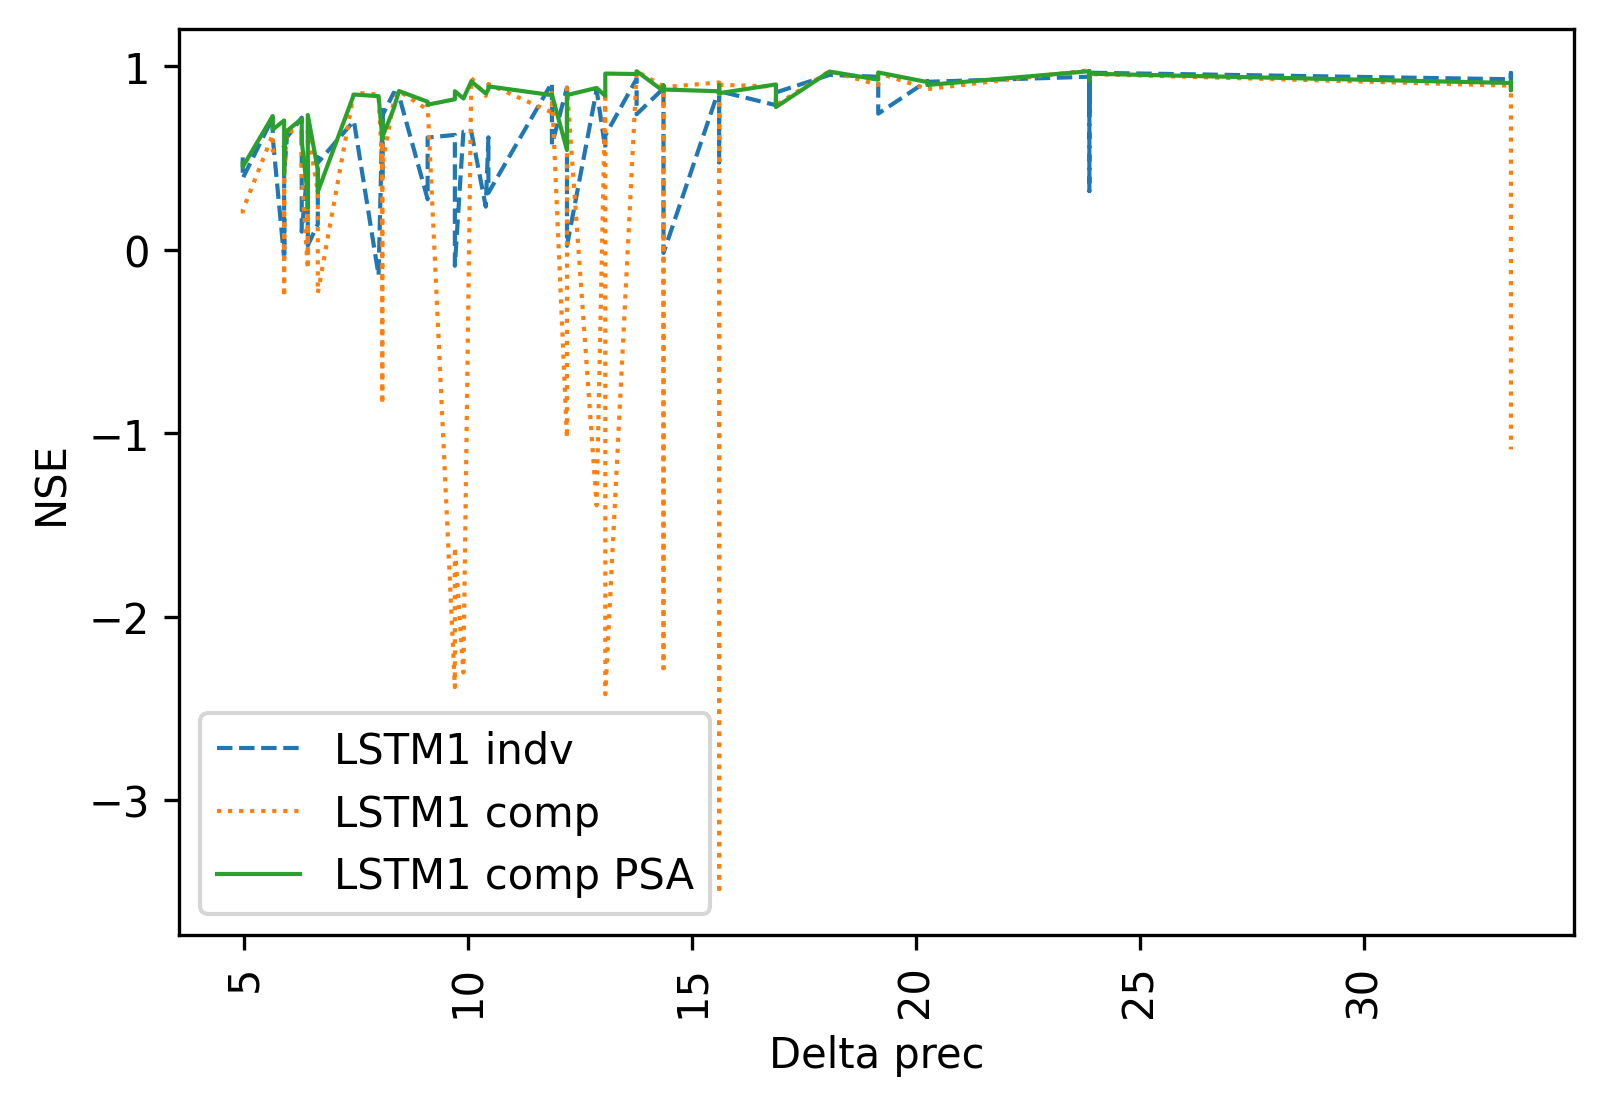
\includegraphics[height=2.in]{Figures/NSEs_Delta prec.png}
% %       \caption{ Modelo LSTM 2}
% %       \label{Red_LSTM2}
% %     \end{center}
% %   \end{figure}

% \section{Resultados finales}

% Con el fin de determinar si los resultados obtenidos utilizando redes neuronales pueden ser utilizados en un problema real 
% de gestión de suministros en una cuenca, se ha alimentado el programa Modsim con los caudales simulados por 
% el modelo hidrológico LEM y los caudales obtenidos por el modelo LSTM1 en el conjunto de test. 
% Se han considerado los diferentes usos del agua por demandas humanas, riego, industriales, etc.
% Los resultados para la salida de la cuenca, se muestran en la figura \ref{modsim}. 
% Se puede apreciar que los resultados son prácticamente iguales.



%   \begin{figure}[h!]
%     \begin{center}
%       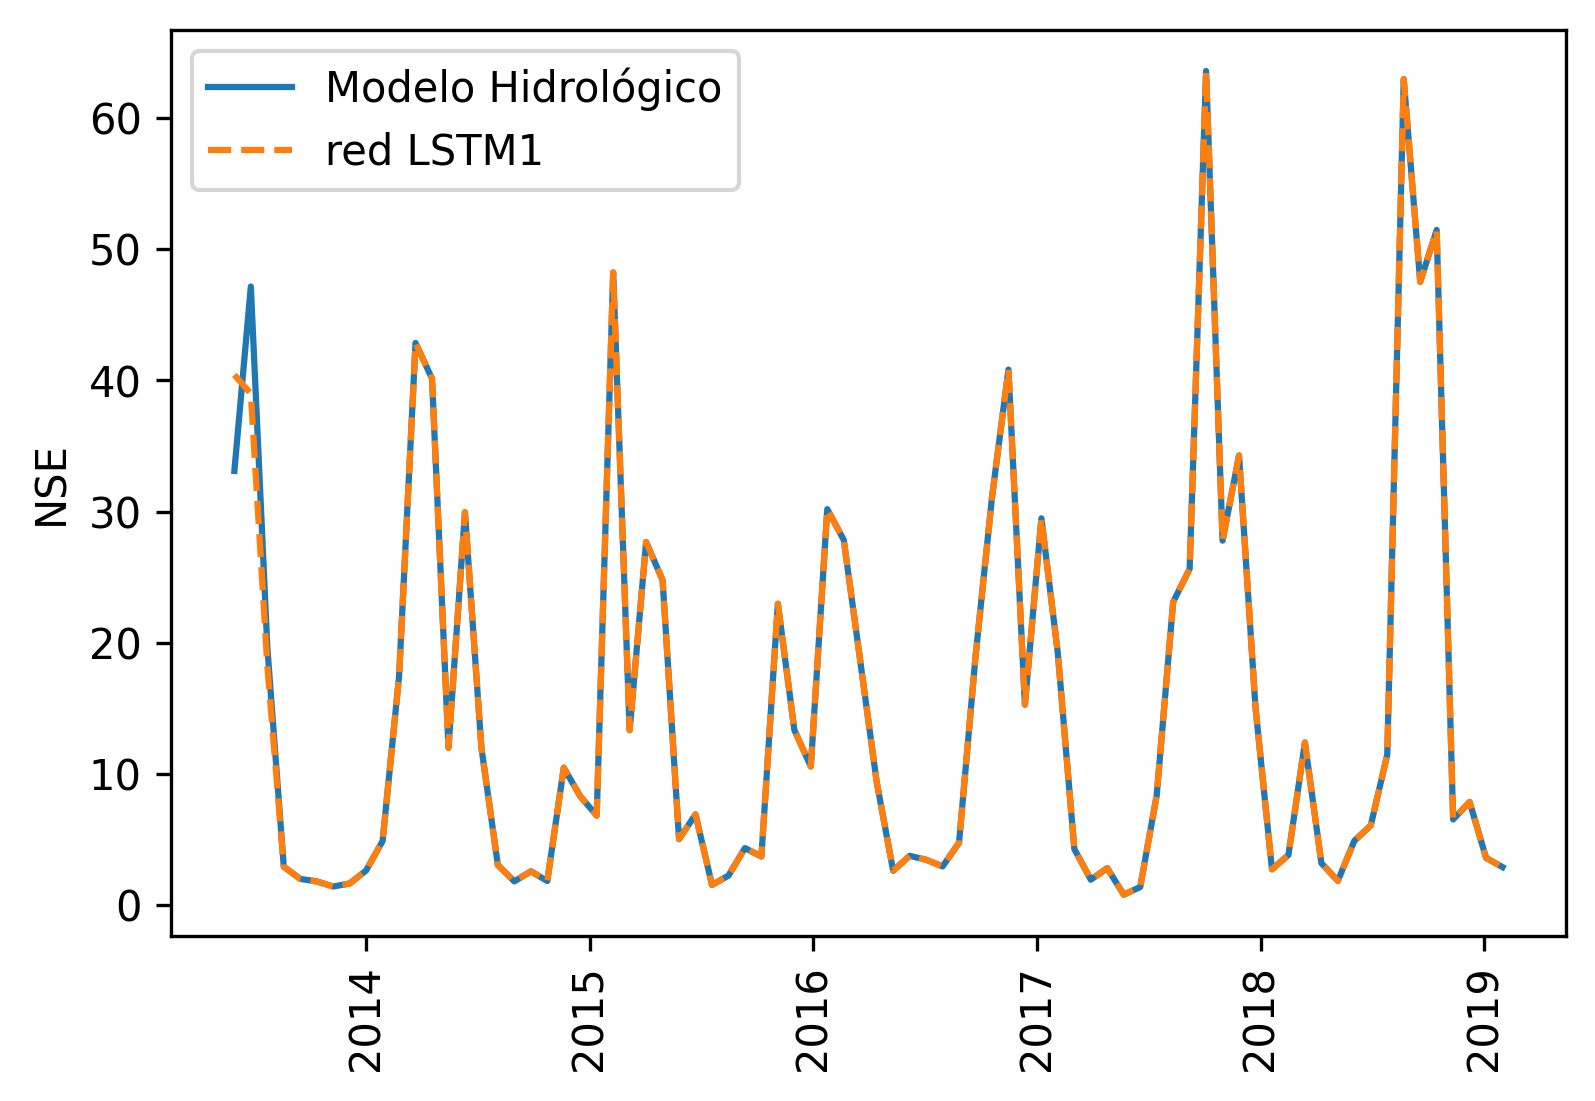
\includegraphics[height=4.in]{Figures/Resultado Modsim.png}
%       \caption{ Resultados finales obtenidos utilizando el software de gestión de recursos Modsim, teniendo en cuenta los usos del agua}
%       \label{modsim}
%     \end{center}
%   \end{figure}


%   % \begin{figure}
% %     \centering
% %     \begin{subfigure}[b]{0.6\textwidth}
% %         \centering
% %         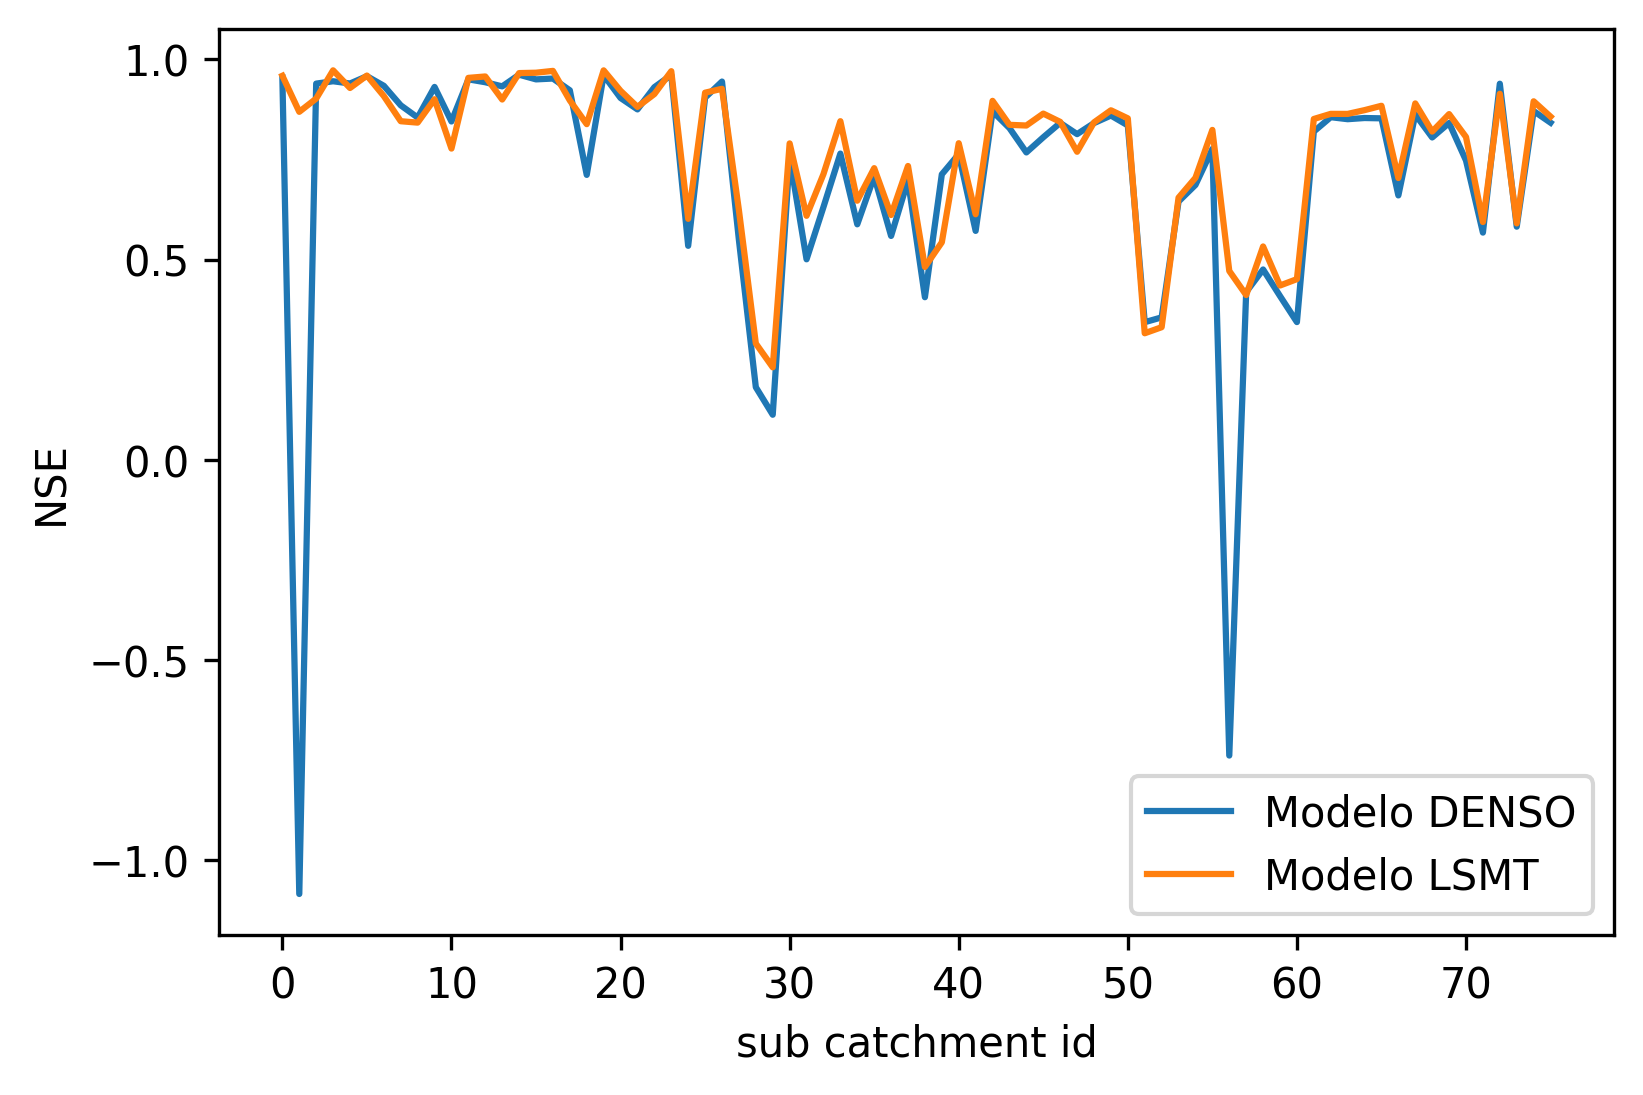
\includegraphics[width=\textwidth]{Figures/comparacion_denso_LSTM_NSE.png}
% %         \caption{}
% %         \label{fig:y equals x}
% %     \end{subfigure}
% %     \hfill
% %     \begin{subfigure}[b]{0.6\textwidth}
% %         \centering
% %         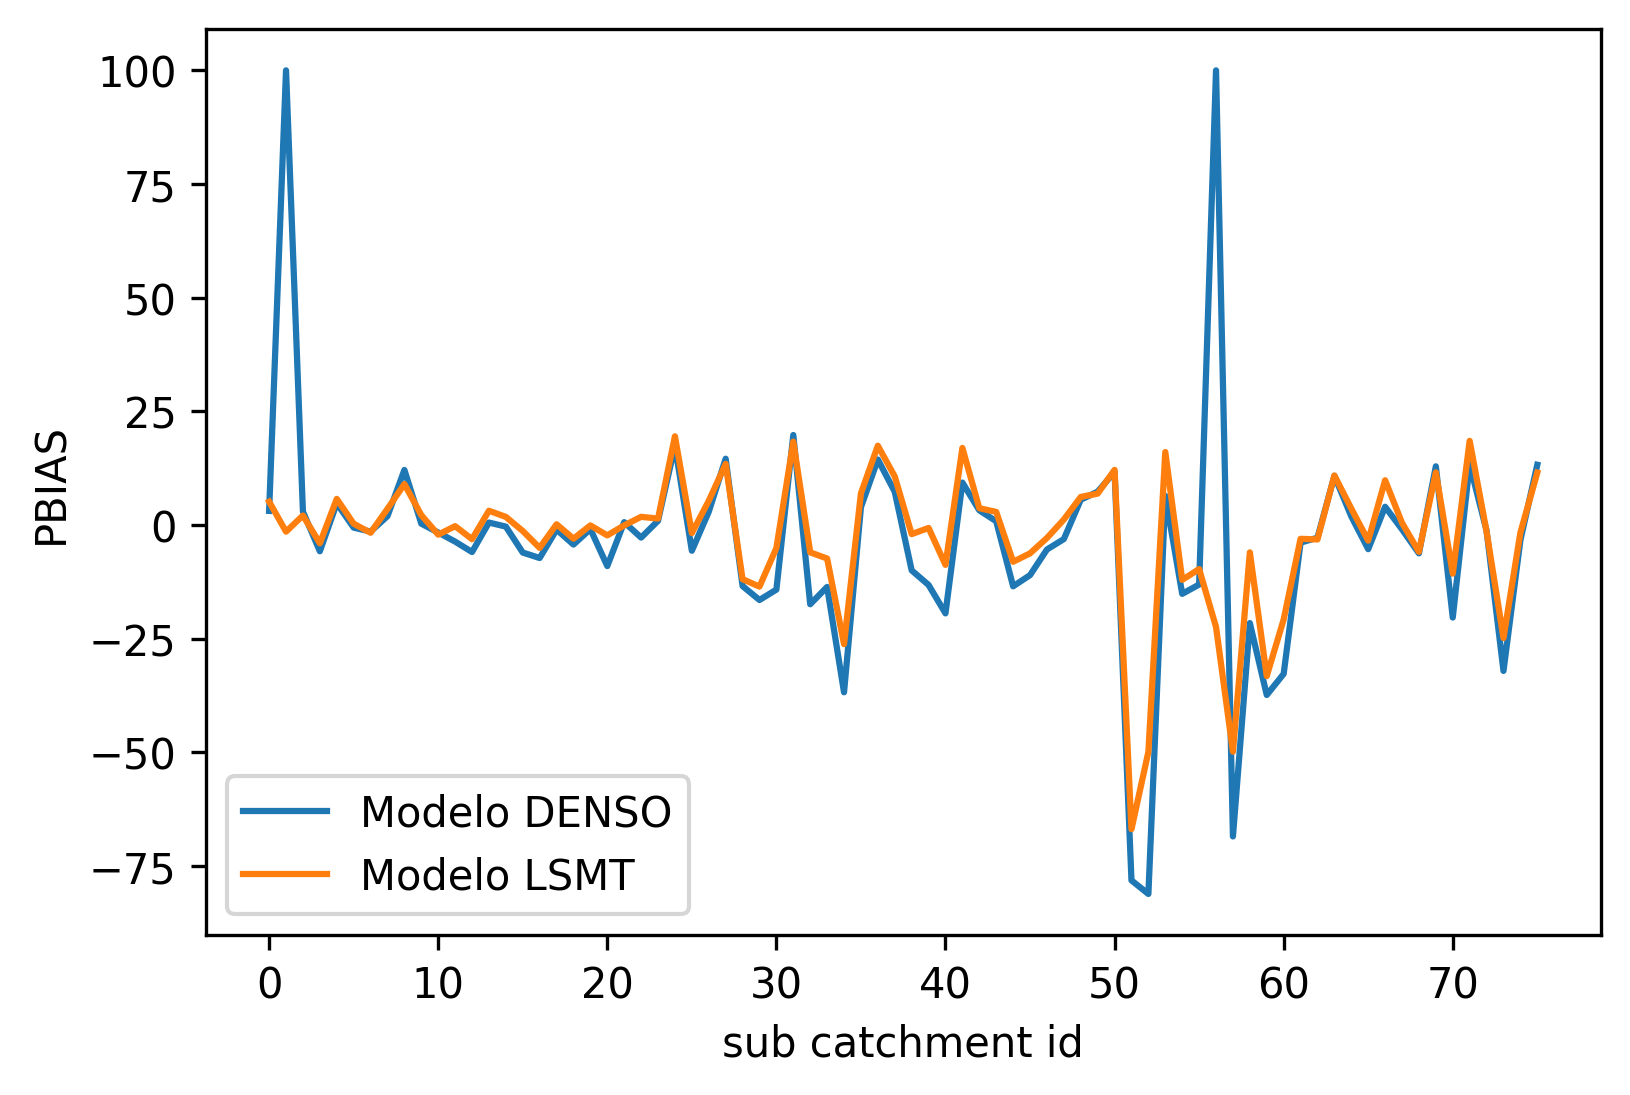
\includegraphics[width=\textwidth]{Figures/comparacion_denso_LSTM_PBIAS.png}
% %         \caption{}
% %         \label{fig:three sin x}
% %     \end{subfigure}
% %        \caption{Three simple graphs}
% %        \label{fig:three graphs}
% % \end{figure}
